\documentclass[a4paper]{article}

\usepackage[italian]{babel}
\usepackage[utf8]{inputenc}
\usepackage{amsmath}
\usepackage{graphicx}
\usepackage[colorinlistoftodos]{todonotes}
\usepackage{csquotes}
\usepackage{hyperref}
\usepackage{float}

\title{%
  Web Information Management \\
  \large Analisi di usabilità di un sito web}

\author{Marco Casagrande - Matricola 1049532}

\date{\today}

\begin{document}
\maketitle

\begin{abstract}
\noindent
Analisi di usabilità di un sito Web, corso di Web Information Management, anno 2016-2017.
\end{abstract}

\newpage
\tableofcontents

\newpage
\section{Introduzione e scopo del documento}

Nei tempi moderni, Internet è un mezzo di comunicazione incredibilmente potente e capillare. Tuttavia non basta possedere delle informazioni per ottenere un pubblico, ma occorre considerare anche la forma e le modalità di accesso.
\\
Parlando di usabilità, è bene partire dalla sua definizione, tratta da un articolo\cite{usab} della Web Accessibility Initiative (WAI):

\begin{quotation}
‘Usability and user experience design is about designing products to be effective, efficient, and satisfying. Specifically, ISO defines usability as the “extent to which a product can be used by specified users to achieve specified goals effectively, efficiently and with satisfaction in a specified context of use" (in ISO 9241-11).’
\end{quotation}

Questo documento si prefigge lo scopo di fornire un'analisi di usabilità del dominio \url{https://www.docker.com}, in data 23 Giugno 2017.

\begin{figure}[H]
	\centering
	
\includegraphics[width=0.5\linewidth]{images/dockerlogo.jpg}
    \label{fig:logodocker}
	\caption{Logo Docker}
\end{figure}

\noindent Il sito in questione promuove il proprio prodotto, chiamato appunto Docker, utilizzato per il deployment di applicazioni. Ciò che lo rende interessante agli occhi degli sviluppatori, è la sua capacità di garantire alle applicazioni l'indipendenza dal sistema di sviluppo, la sicurezza e la scalabilità.

\section{Analisi preliminare}

\subsection{Contesto}
Docker è un ambiente di sviluppo per il deployment di applicazioni.
Il suo ambito è molto specifico e la sua utenza sarà altamente specializzata. Chiunque non sia uno sviluppatore non sarà interessato a Docker e probabilmente nemmeno nessun neofita informatico sarebbe in grado di sfruttarne le funzionalità. Nonostante l'esperienza dell'utente medio sia molto influente nel valutare, essa non costituisce una scusa per eventuali lacune nell'usabilità.
\\
Lo scopo principale del sito è promuovere il proprio prodotto, esponendo una panoramica generale delle proprie features. Uno scopo secondario è fornire un portale d'accesso alla documentazione ed alla community di Docker.

\subsection{Nome del dominio}
Il nome è un fattore molto importante ed è consigliabile seguire alcune linee guida nella sua scelta.

Il nome \textbf{Docker} è:
\begin{itemize}
	\item correttamente registrato e/o in attesa di approvazione (controllo eseguito a nome "Docker" e genere "software" tramite il sito \url{http://www.wipo.int/branddb/en/});
    \item unico;
    \item corto;
    \item facile da memorizzare e da scrivere;
    \item riutilizza la parola inglese dock (porto);
    \item seguito dal dominio ".com".
\end{itemize}

Il nome Docker rispetta gran parte delle linee guida rivelandosi un'ottima scelta.

\section{Homepage}

\subsection{Descrizione generale}
L'analisi dell'homepage di \url{https://www.docker.com/}, dato il moderato sviluppo in verticale, sarà effettuata descrivendo i singoli screen.

\begin{figure}[H]
	\centering
	
\includegraphics[width=\linewidth]{images/homepage1.png}
    \label{fig:homepage1}
    \caption{Homepage screen 1}
\end{figure}

\noindent La parte più importante dell'homepage, visibile senza scroll. Si possono notare alcuni elementi importanti e ricorrenti nei siti web, come:

\begin{itemize}
	\item il logo in alto a sinistra;
    \item la breadcrumb per la navigazione all'interno del sito;
    \item la vetrina delle novità riguardanti il prodotto, che cambiano ad intervalli regolari;
    \item una gradevole palette blu e bianca, che risulta ben leggibile agli utenti;
    \item la breadcrumb per la navigazione all'interno della pagina;
    \item il contenuto della pagina.
\end{itemize}

\begin{figure}[H]
	\centering
	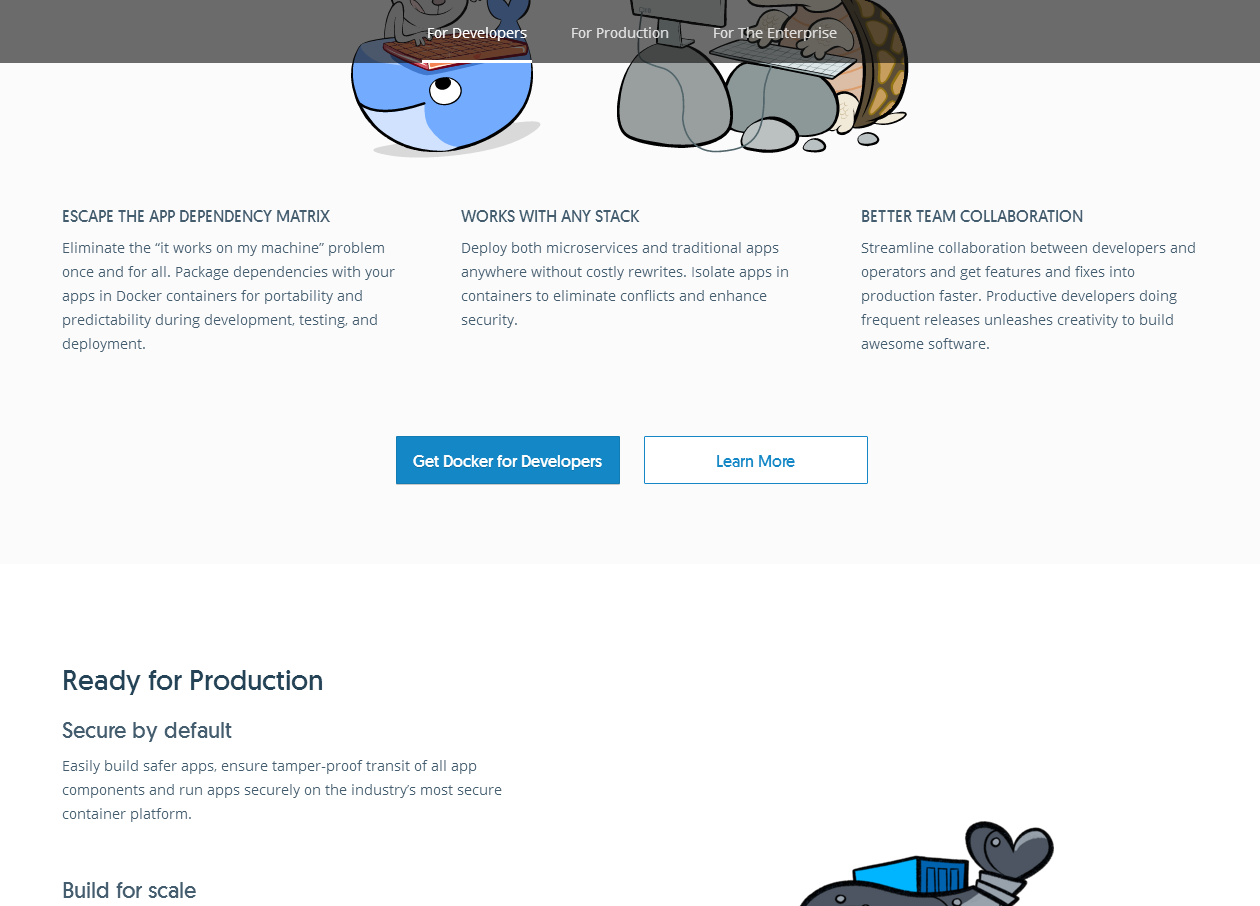
\includegraphics[width=\linewidth]{images/homepage2.png}
    \label{fig:homepage2}
    \caption{Homepage screen 2}
\end{figure}

\noindent Il contenuto della pagina consiste in immagini, paragrafi di testo (contenuti generali), colonne di testo (contenuti più specifici) e vari link a pagine interne al sito, accessibili tramite intuitivi pulsanti.

\begin{figure}[H]
	\centering
	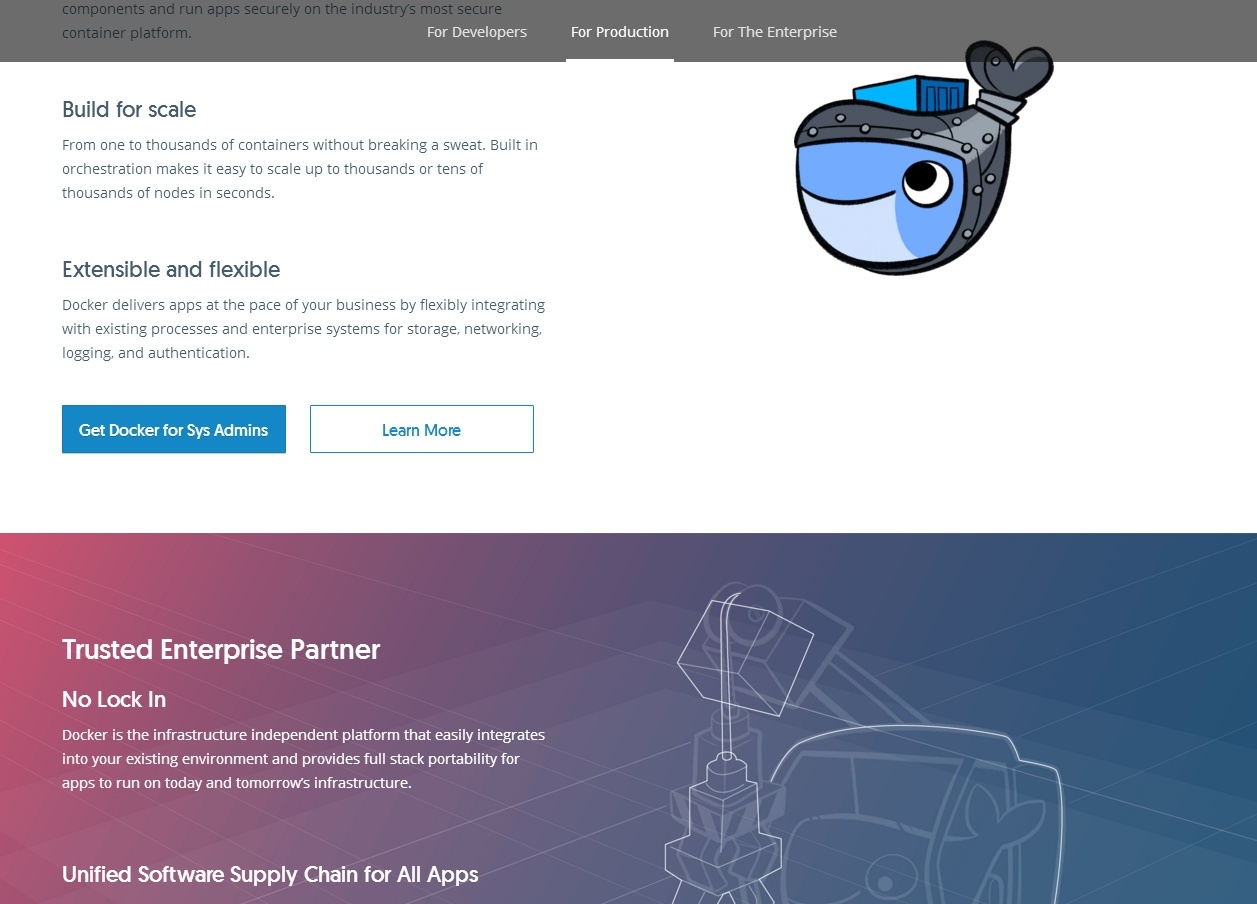
\includegraphics[width=\linewidth]{images/homepage3.jpg}
    \label{fig:homepage3}
    \caption{Homepage screen 3}
\end{figure}

\begin{figure}[H]
	\centering
	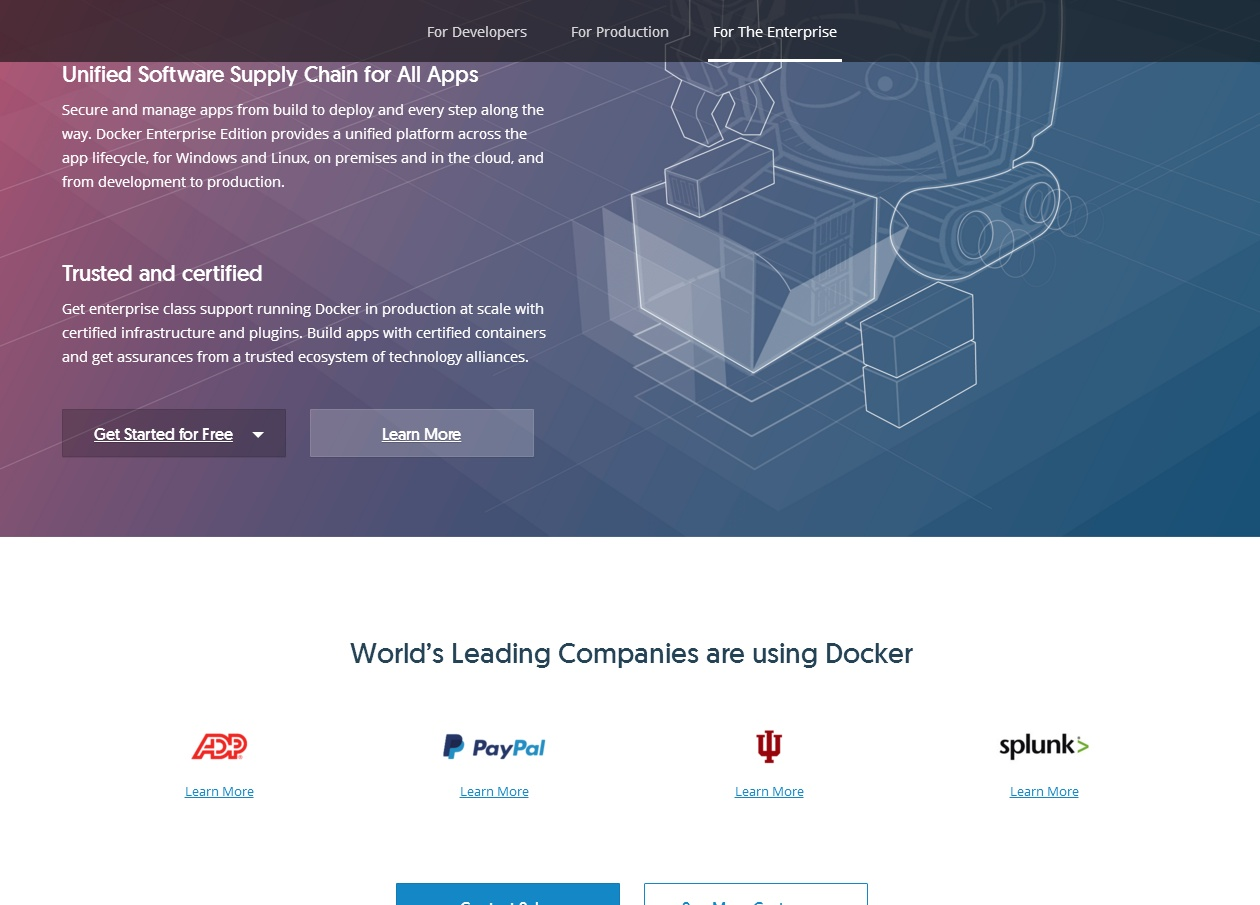
\includegraphics[width=\linewidth]{images/homepage4.jpg}
    \label{fig:homepage4}
    \caption{Homepage screen 4}
\end{figure}

\noindent Verso la fine della pagina compare la lista delle compagnie più famose che usano Docker.

\begin{figure}[H]
	\centering
	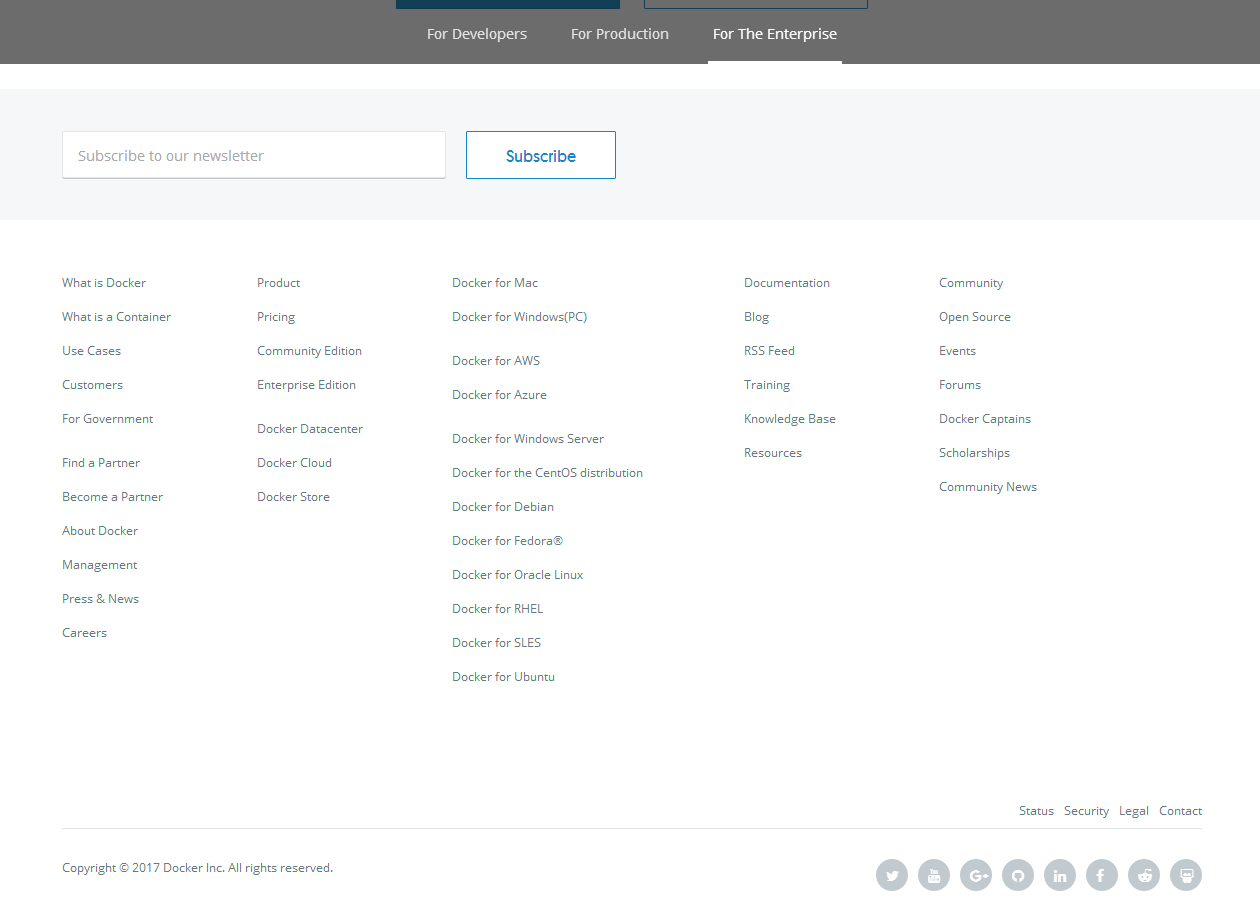
\includegraphics[width=\linewidth]{images/homepage5.png}
    \label{fig:homepage5}
    \caption{Homepage screen 5}
\end{figure}

\noindent Nel footer sono incluse ogni genere di informazioni, che coprono qualsiasi pagina e settore coperto dal sito.

\newpage
\subsection{The Six Ws}
Il miglior modo per valutare l'impatto sul visitatore del sito, è analizzare le cosiddette "Six Ws".

\subsubsection{Where?}
La domanda "Where?" corrisponde ad "In che sito mi trovo?".

\begin{figure}[H]
	\centering
	
\includegraphics[width=\linewidth]{images/where.png}
    \label{fig:homepagewhere}
    \caption{Individuazione Where in homepage}
\end{figure}

\noindent La risposta non è immediata. Docker gode di una certa fama, ma non a tal punto da non aver bisogno di presentazioni. Per buona parte dell'utenza, nome e logo non aiutano minimamente a capire che prodotto venga presentato.
\\
Tra le quattro novità che scorrono regolarmente, solo quella mostrata in figura descrive minimamente il prodotto. Difficilmente l'utente si fermerà a leggerli tutti, nella speranza di trovare qualche suggerimento, probabilmente osserverà solo il primo.
\\
La breadcrumb per la navigazione interna alla pagina offre degli spunti con le parole "Developers" e "Production". I termini sono però così generici da non poter venire collegati immediatamente all'ambito informatico.
\\
Lo slogan "A Better Way to Build Apps" è dunque l'unico indizio utile a capire la natura del sito ed è decisamente insufficiente.
\\
Anche il contenuto della pagina è insoddisfacente in questo ambito. Infatti si limita a descrivere i pregi dell'utilizzo di Docker, senza definirlo a chiare lettere un "ambiente di sviluppo per il deployment di applicazioni".
\\
La lista delle compagnie che impiegano Docker permette di capire che si tratta di un prodotto informatico, ma solo nel caso si conoscano tali compagnie e solo se l'utente ha deciso di scorrere così in basso la pagina.
\\
Queste informazioni mancanti sono invece ben esposte nella pagina \url{https://www.docker.com/what-docker}, ma ciò non toglie la grave mancanza della homepage nel rispondere alla domanda Where. 

\subsubsection{Who?}
La domanda "Who?" corrisponde a "Chi rappresenta il sito?".

\begin{figure}[H]
	\centering
	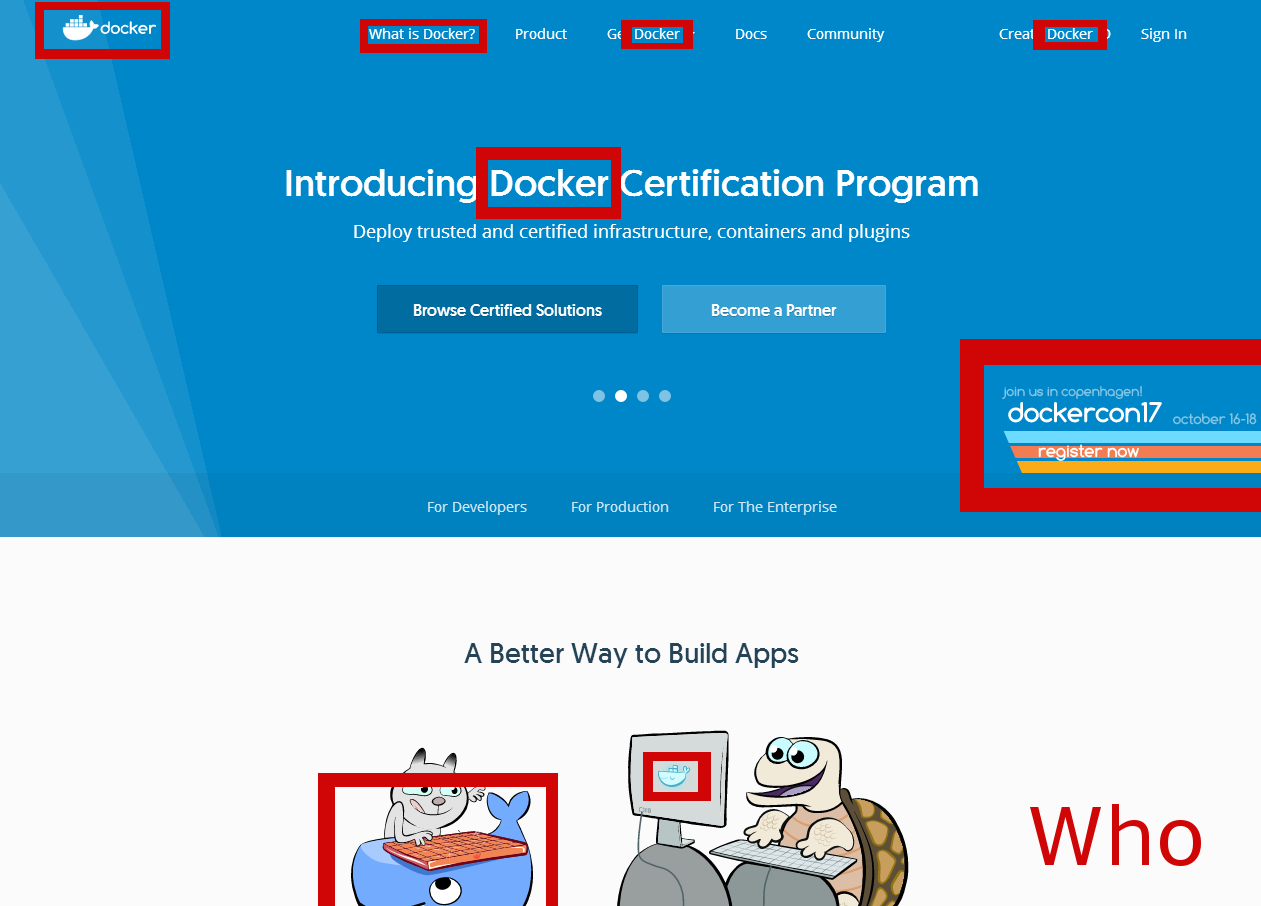
\includegraphics[width=\linewidth]{images/who.png}
    \label{fig:homepagewho}
    \caption{Individuazione Who in homepage}
\end{figure}

\noindent La risposta è immediata. Sono presenti numerosi richiami sia al nome Docker che al logo della balena. L'identità della compagnia è ben definita nei colori blu e bianco, nel logo e nella metafora del porto (dock) rintracciabile in molte immagini.
\\
Anche se è difficile intuire cosa sia Docker, sicuramente è facile memorizzarne e riconoscerne nome e logo.

\subsubsection{Why?}
La domanda "Why?" corrisponde a "Perchè sono qui? Quali benefici ottengo dal sito?".

\begin{figure}[H]
	\centering
	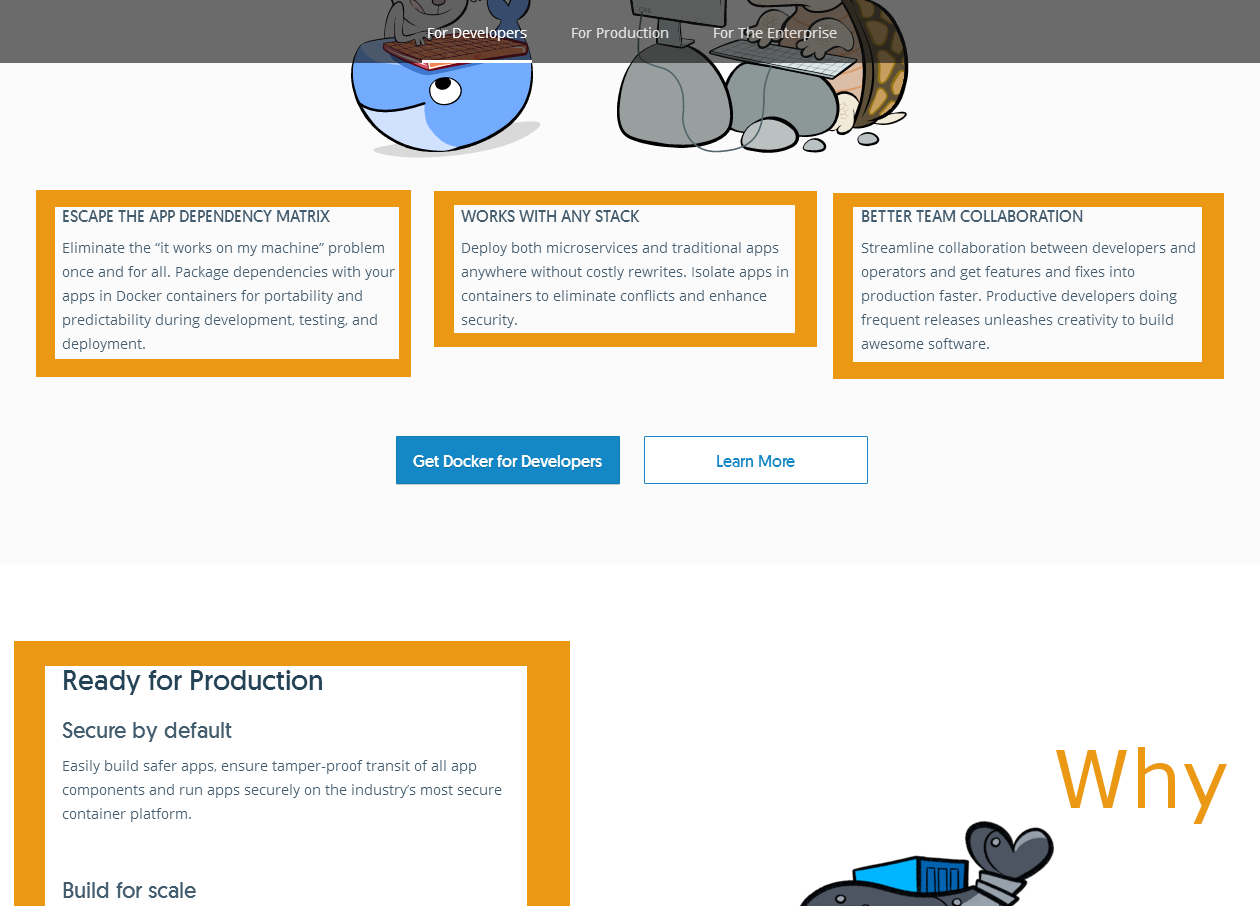
\includegraphics[width=\linewidth]{images/why.png}
    \label{fig:homepagewhy}
    \caption{Individuazione Why in homepage}
\end{figure}

\noindent La risposta è chiara, a patto di scorrere brevemente. Gli sviluppatori di Docker hanno trovato numerosissime motivazioni per usare il loro software ed il sito ne è letteralmente cosparso. 
\\
I paragrafi esplicativi sono ben distribuiti nello spazio e si può intuire facilmente quali contengano informazioni generiche e quali specifiche. Questo schema organizzativo viene ripreso in tutto il sito e l'utente ci si abitua rapidamente.
\\
La lista delle compagnie più famose che utilizzano Docker conferisce un bonus per l'autorevolezza del prodotto: se lo usa PayPal, sicuramente avrà i suoi motivi no?

\newpage
\subsubsection{What?}
La domanda "What?" corrisponde a "Cosa viene offerto dal sito?".

\begin{figure}[H]
	\centering
	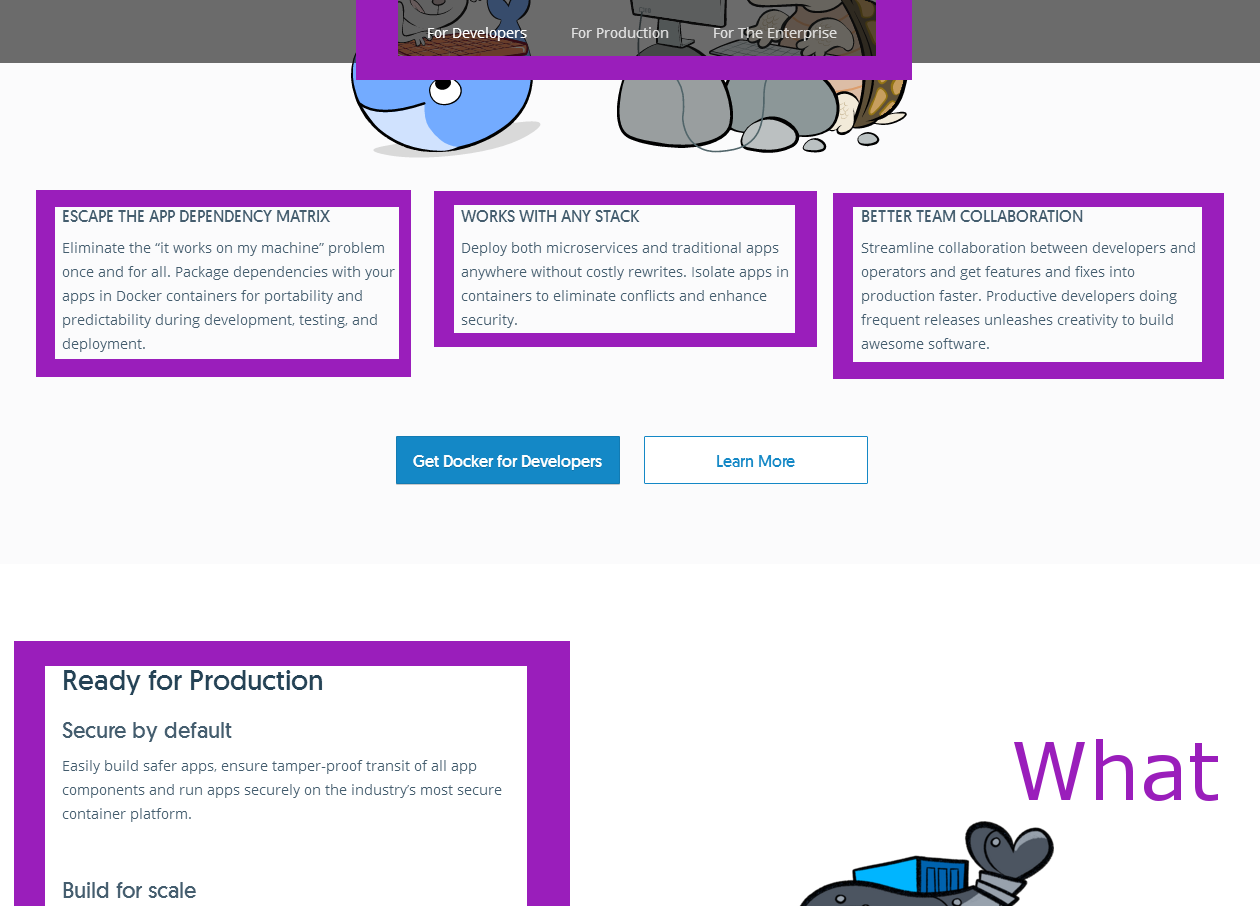
\includegraphics[width=\linewidth]{images/what.png}
    \label{fig:homepagewhat}
    \caption{Individuazione What in homepage}
\end{figure}

\noindent La risposta non è chiara. La radice del problema deriva dall'incapacità di comprendere in cosa consista il prodotto. Al contrario, i benefici che esso porta sono molteplici e ben elaborati.
\\
Questo provoca un senso di disorientamento durante la navigazione della homepage. L'utente può trovare tutte le informazioni che vuole tranne quella più importante.

\newpage
\subsubsection{When?}
La domanda "When?" corrisponde a "Quali sono le ultime novità del sito?".

\begin{figure}[H]
	\centering
	
\includegraphics[width=\linewidth]{images/when.png}
    \label{fig:homepagewhen}
    \caption{Individuazione When in homepage}
\end{figure}

\noindent La risposta è immediata. La vetrina della novità riempie una gran parte della schermata iniziale della homepage (forse anche troppo).
\\
La vetrina ha (attualmente) quattro novità che si alternano regolarmente ed espongono notizie di vario genere affini a Docker. Alcune riportano anche la data (sarebbe consigliabile riportarla su tutte) e tutte presentano almeno un link per l'approfondimento.
\\
Un altro elemento che compare nella vetrina, anche se non ne fa propriamente parte, è l'invito a partecipare al Dockercon17 (con data e luogo riportati).
\\
Nonostante il buon layout impiegato, il sito non sembra particolarmente dinamico. Vista la natura del prodotto, certamente non ci si può aspettare novità quotidianamente, ma un avviso riguardante l'ultima versione rilasciata che rimandi al changelog, conferirebbe a Docker un'aspetto di software attivo ed in costante aggiornamento.
\\
L'invito per il Dockercon17 riesce a risollevare un po' le aspettative (a patto di non sapere che la homepage è identica da molti mesi, come pure l'invito).

\newpage
\subsubsection{How?}
La domanda "How?" corrisponde a "Come arrivo alle sezioni principali del sito?".

\begin{figure}[H]
	\centering
	
\includegraphics[width=\linewidth]{images/how1.png}
    \label{fig:homepagehow1}
    \caption{Individuazione How in homepage}
\end{figure}

\begin{figure}[H]
	\centering
	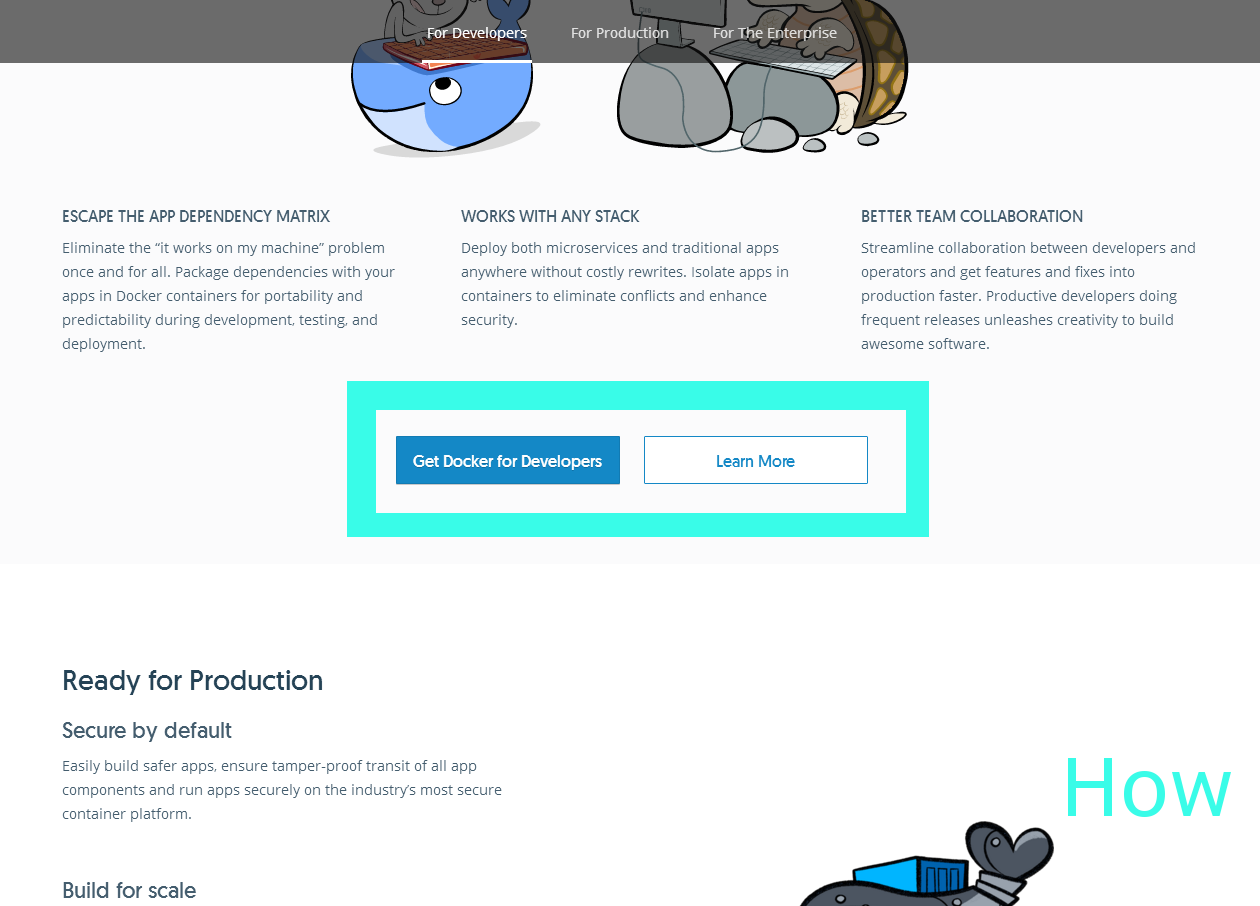
\includegraphics[width=\linewidth]{images/how2.png}
    \label{fig:homepagehow2}
    \caption{Individuazione How in homepage}
\end{figure}

\begin{figure}[H]
	\centering
	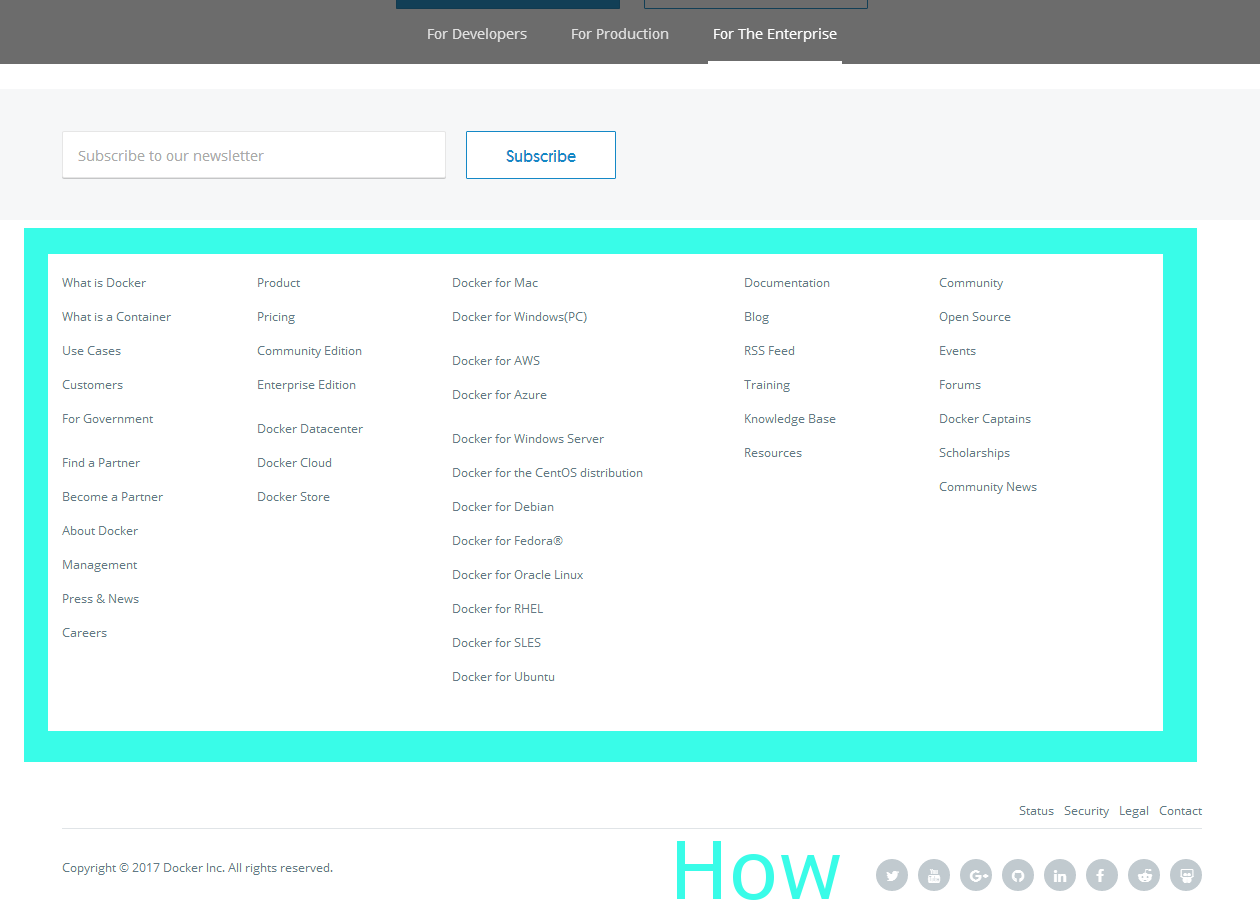
\includegraphics[width=\linewidth]{images/how3.png}
    \label{fig:homepagehow3}
    \caption{Individuazione How in homepage}
\end{figure}

\noindent La risposta è chiara. Sono presenti vari elementi per illustrare la struttura del sito.
\\
La breadcrumb in alto al centro presenta le sezioni principali del sito ed è sempre presente.
\\
La breadcrumb centrale presenta le sezioni principali della pagina corrente e segue l'utente nello scorrimento verticale.
\\
I pulsanti offrono scorciatoie verso le pagine interne al sito ed è chiaro l'argomento cui conducono.
\\
Il footer espone l'insieme delle sottosezioni delle pagine interne al sito, incolonnate per sezione. In questo modo l'utente può sempre giungere con un solo click all'argomento desiderato.

\section{Product}

\subsection{Descrizione generale}
L'analisi della pagina product di \url{https://www.docker.com/get-docker}, dato il moderato sviluppo in verticale, sarà effettuata descrivendo i singoli screen.

\begin{figure}[H]
	\centering
	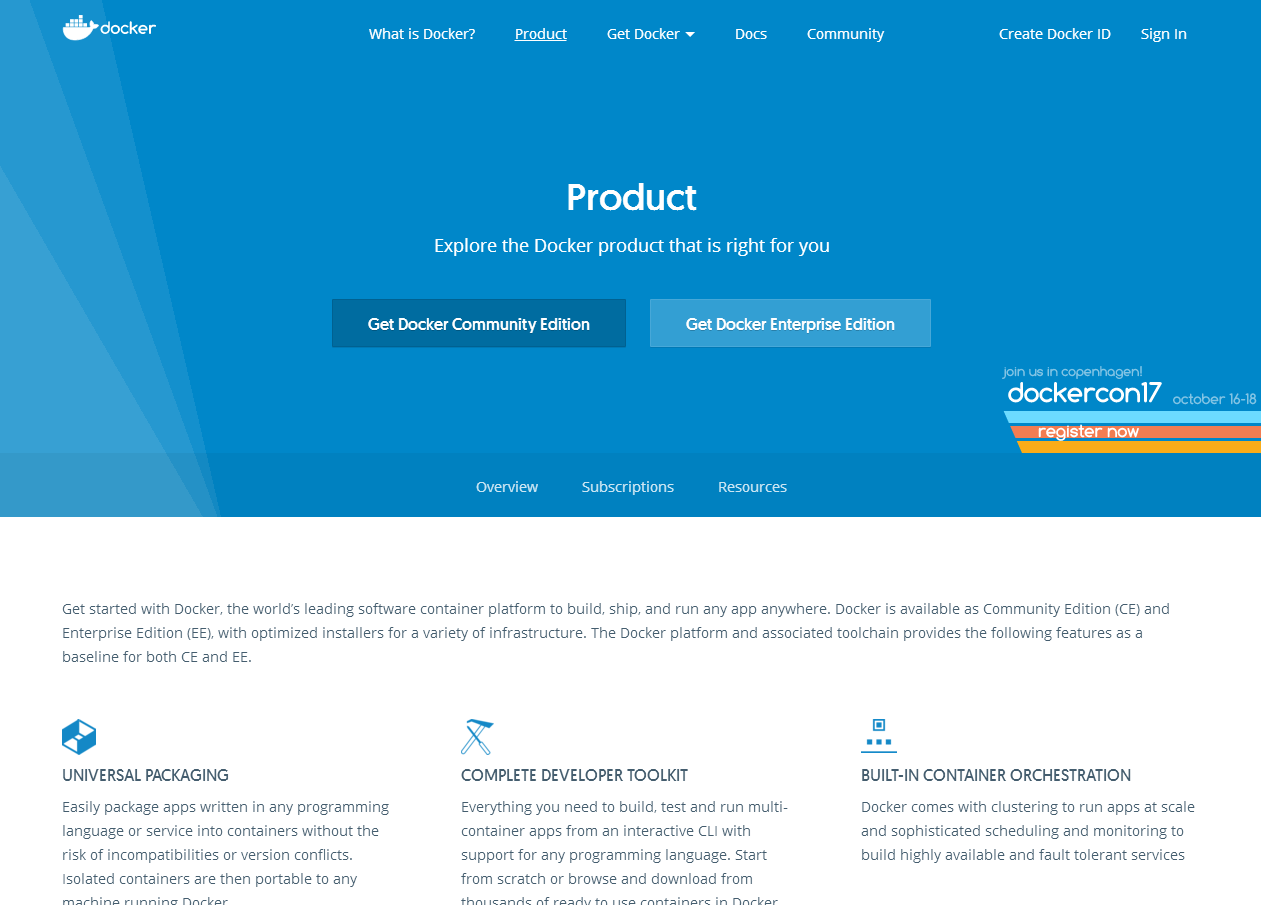
\includegraphics[width=\linewidth]{images/product1.png}
    \label{fig:product1}
    \caption{Product screen 1}
\end{figure}

\noindent La parte superiore della pagina si presenta identica alla homepage, fatta eccezione per la vetrina delle novità che contiene un messaggio leggermente modificato e fisso.

\begin{figure}[H]
	\centering
	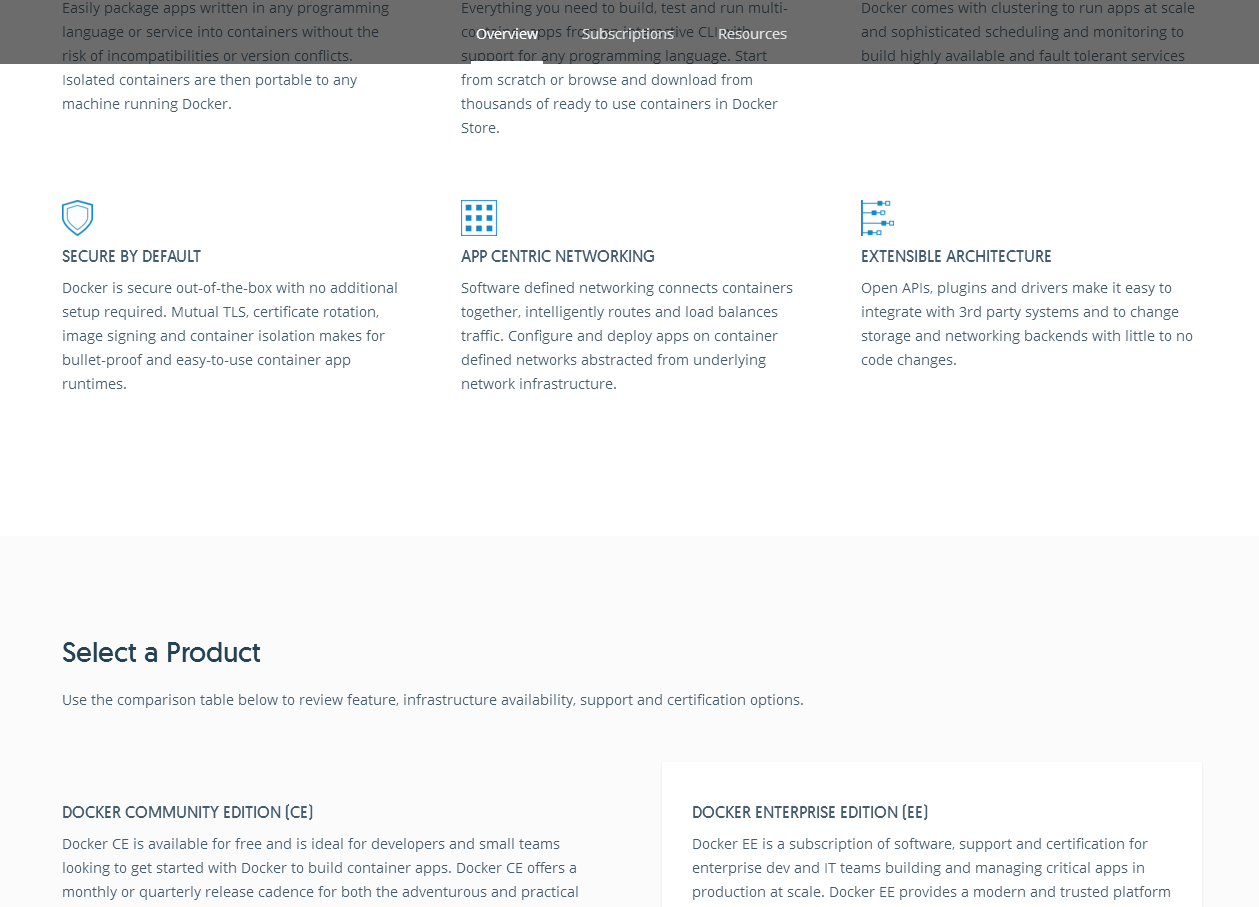
\includegraphics[width=\linewidth]{images/product2.png}
    \label{fig:product2}
    \caption{Product screen 2}
\end{figure}

\noindent Viene presentata una lista di qualità e features di Docker organizzata a mo' di griglia.

\begin{figure}[H]
	\centering
	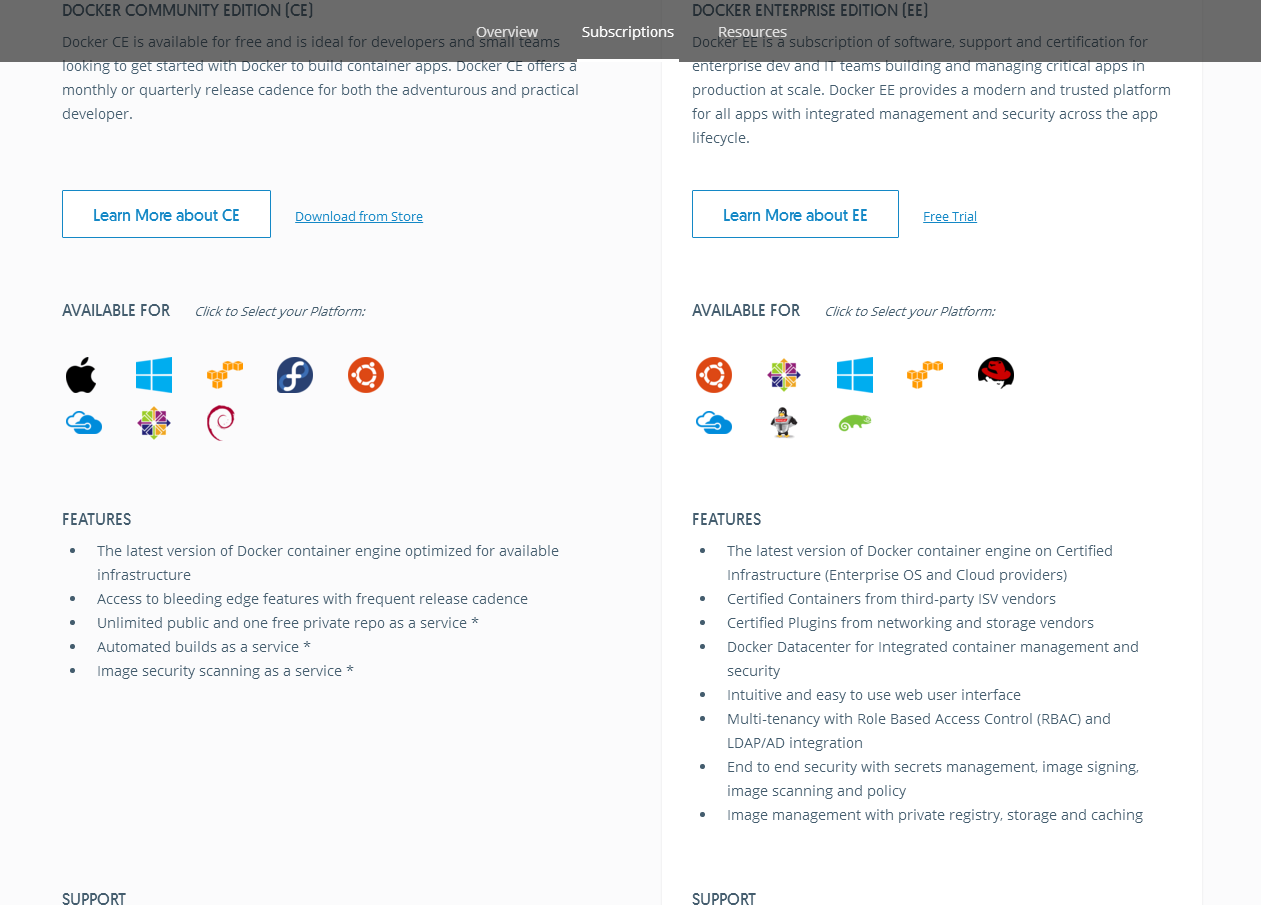
\includegraphics[width=\linewidth]{images/product3.png}
    \label{fig:product3}
    \caption{Product screen 3}
\end{figure}

\noindent Vengono mostrate due colonne (una per developers e team, l'altra per enterprises) che descrivono il contenuto del software scaricabile/acquistabile. Sono presenti varie icone per la scelta della piattaforma.

\begin{figure}[H]
	\centering
	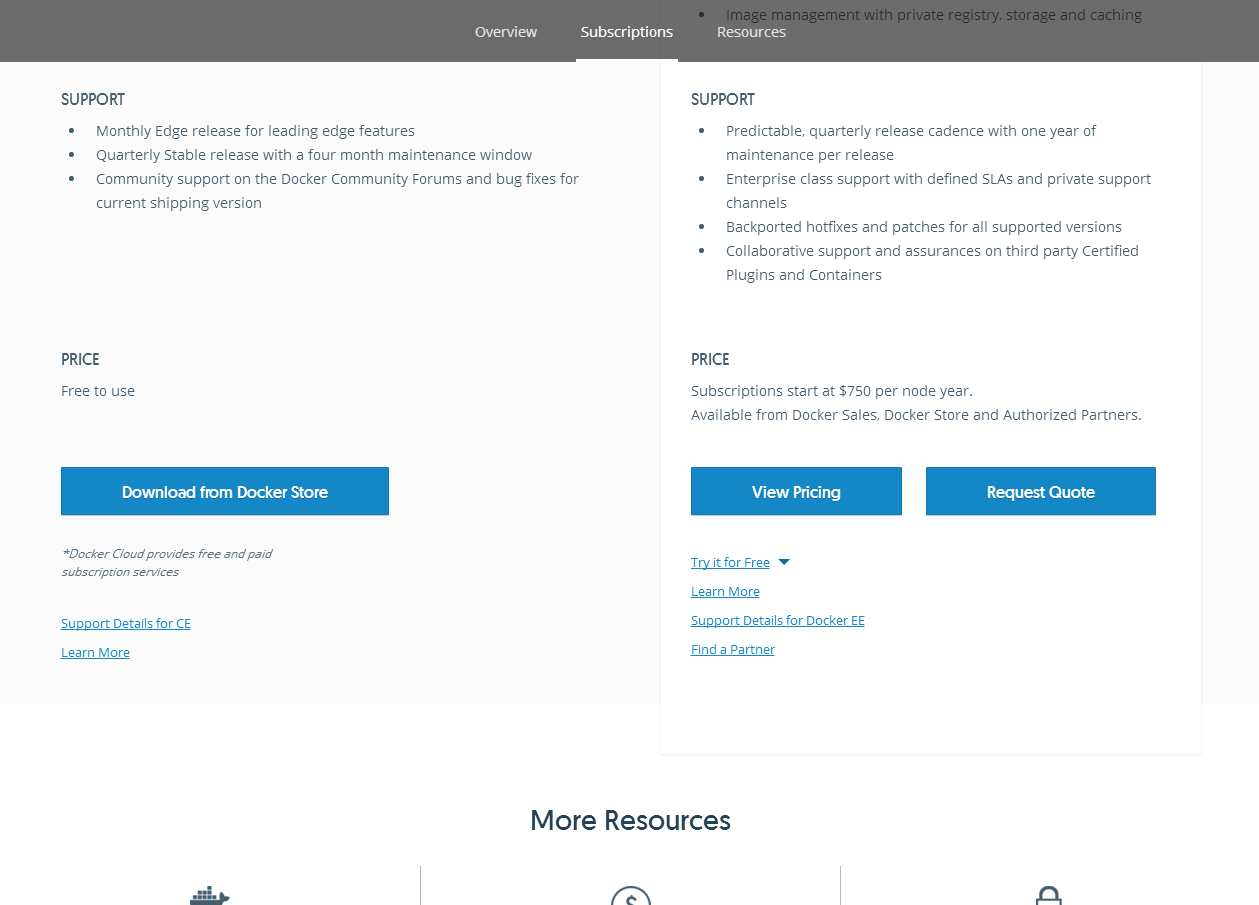
\includegraphics[width=\linewidth]{images/product4.png}
    \label{fig:product4}
    \caption{Product screen 4}
\end{figure}

\noindent Vengono mostrare le informazioni sul prezzo e link per approfondimenti sul software e sul supporto.

\begin{figure}[H]
	\centering
	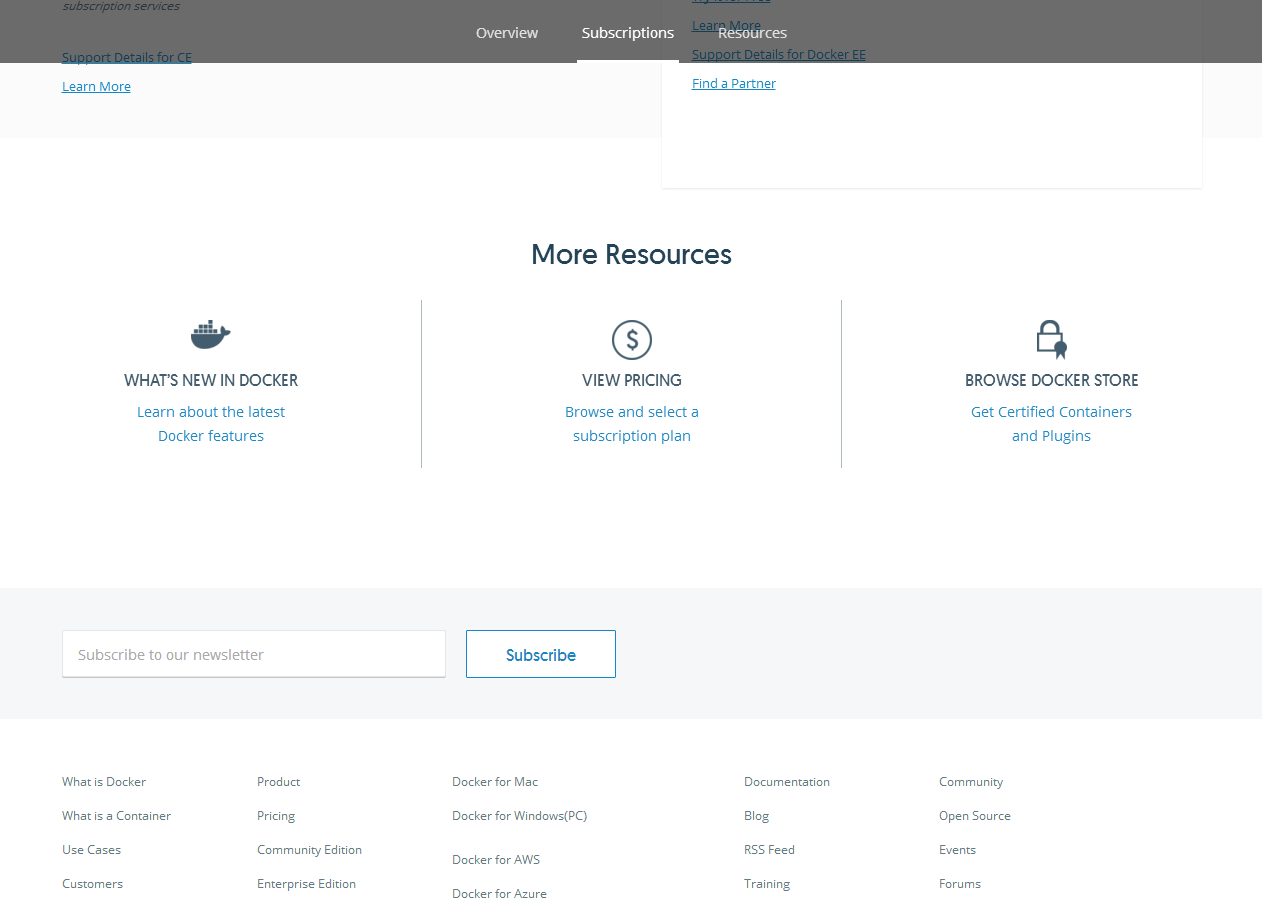
\includegraphics[width=\linewidth]{images/product5.png}
    \label{fig:product5}
    \caption{Product screen 5}
\end{figure}

\noindent Vengono mostrati altri link utili ad esplorare il mondo di Docker.

\begin{figure}[H]
	\centering
	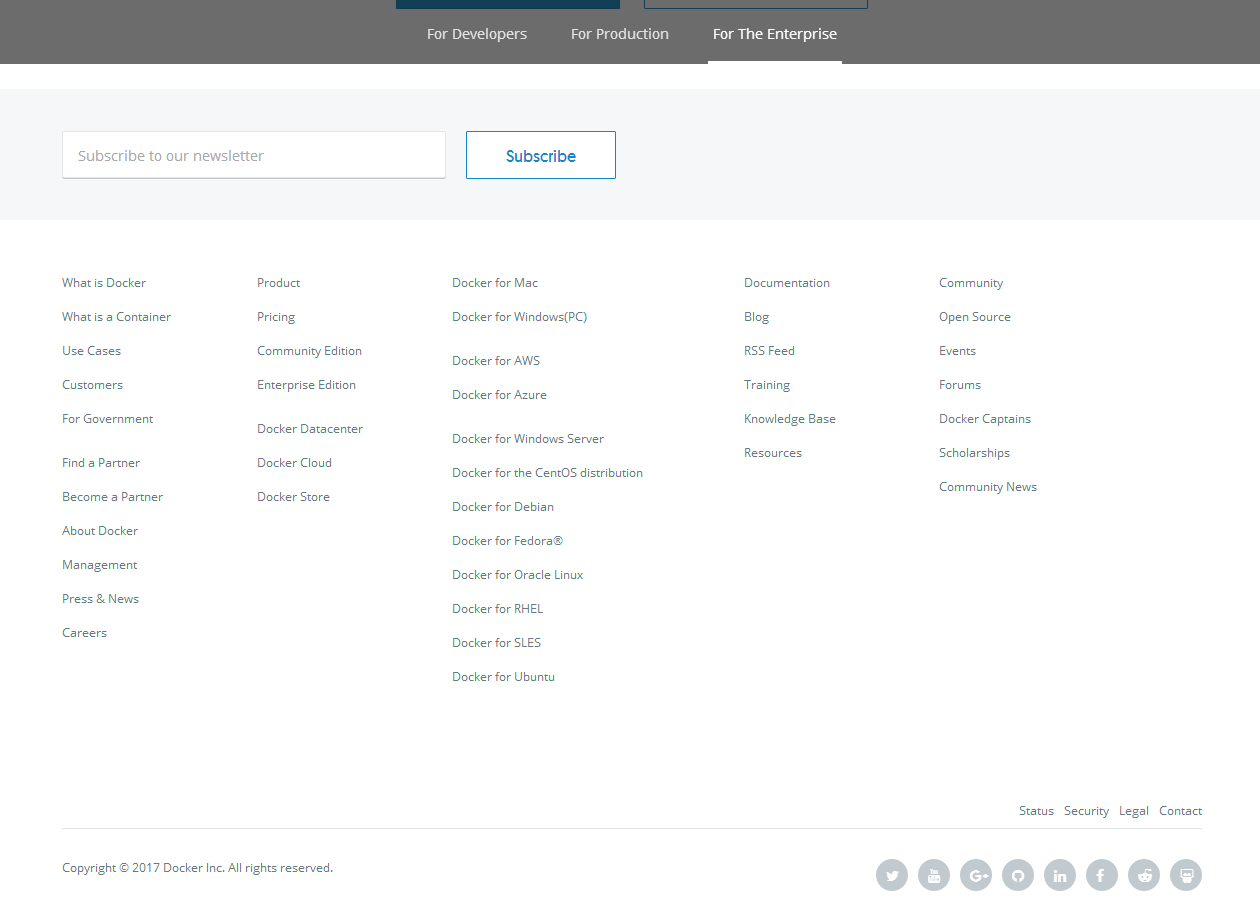
\includegraphics[width=\linewidth]{images/product6.png}
    \label{fig:product6}
    \caption{Product screen 6}
\end{figure}

\subsection{The Six Ws}

\subsubsection{Where?}
La domanda "Where?" corrisponde ad "In che sito mi trovo?".
\\
Nelle pagine interne rispondere a tale domanda è fondamentale.

\begin{figure}[H]
	\centering
	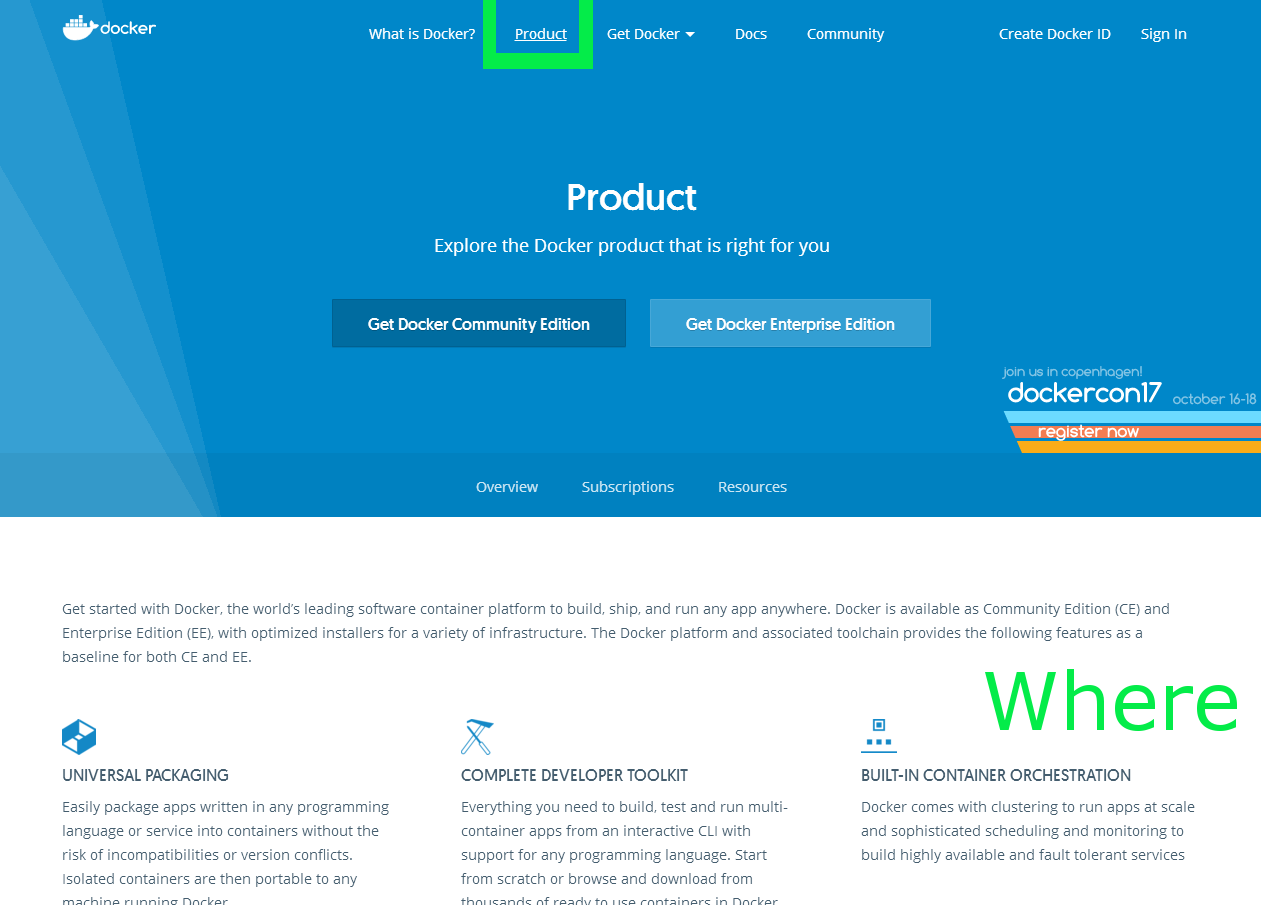
\includegraphics[width=\linewidth]{images/productwhere.png}
    \label{fig:productwhere}
    \caption{Individuazione Where in product}
\end{figure}

\noindent La risposta non è molto chiara. Si può intravedere la sottolineatura della parola "Product" nella breadcrumb in alto al centro, ma è decisamente poco visibile e non vi è alcun altro indicatore.
\\
Si può attribuire questa negligenza alla semplicità del sito, che presenta poche pagine e nessuna veramente interna all'altra. Tuttavia un visitatore non può conoscere l'organizzazione di un sito senza averlo prima navigato, e senza indicazioni si ritroverà disorientato.

\newpage
\subsubsection{Who?}
La domanda "Who?" corrisponde a "Chi rappresenta il sito?".
\\
Nelle pagine interne rispondere a tale domanda è obbligatorio.

\begin{figure}[H]
	\centering
	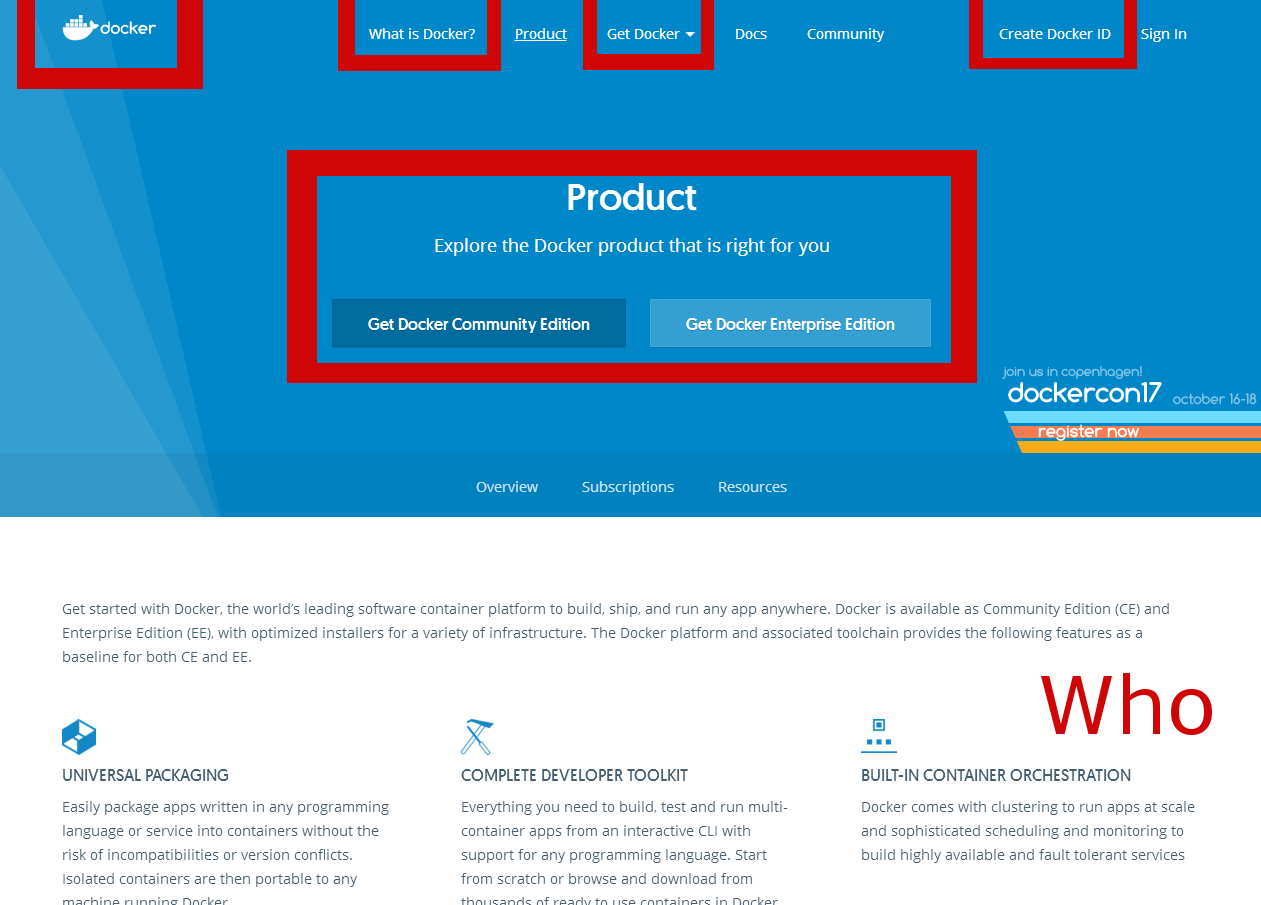
\includegraphics[width=\linewidth]{images/productwho.png}
    \label{fig:productwho}
    \caption{Individuazione Who in product}
\end{figure}

\noindent La risposta è immediata. Come nella homepage, sono presenti molti richiami al nome del prodotto. In alto a sinistra sono presenti (ovunque nel sito) il logo ed il nome, che se clickati riportano alla homepage.

\newpage
\subsubsection{What?}
La domanda "What?" corrisponde a "Cosa viene offerto dal sito?".
\\
Nelle pagine interne rispondere a tale domanda è obbligatorio.

\begin{figure}[H]
	\centering
	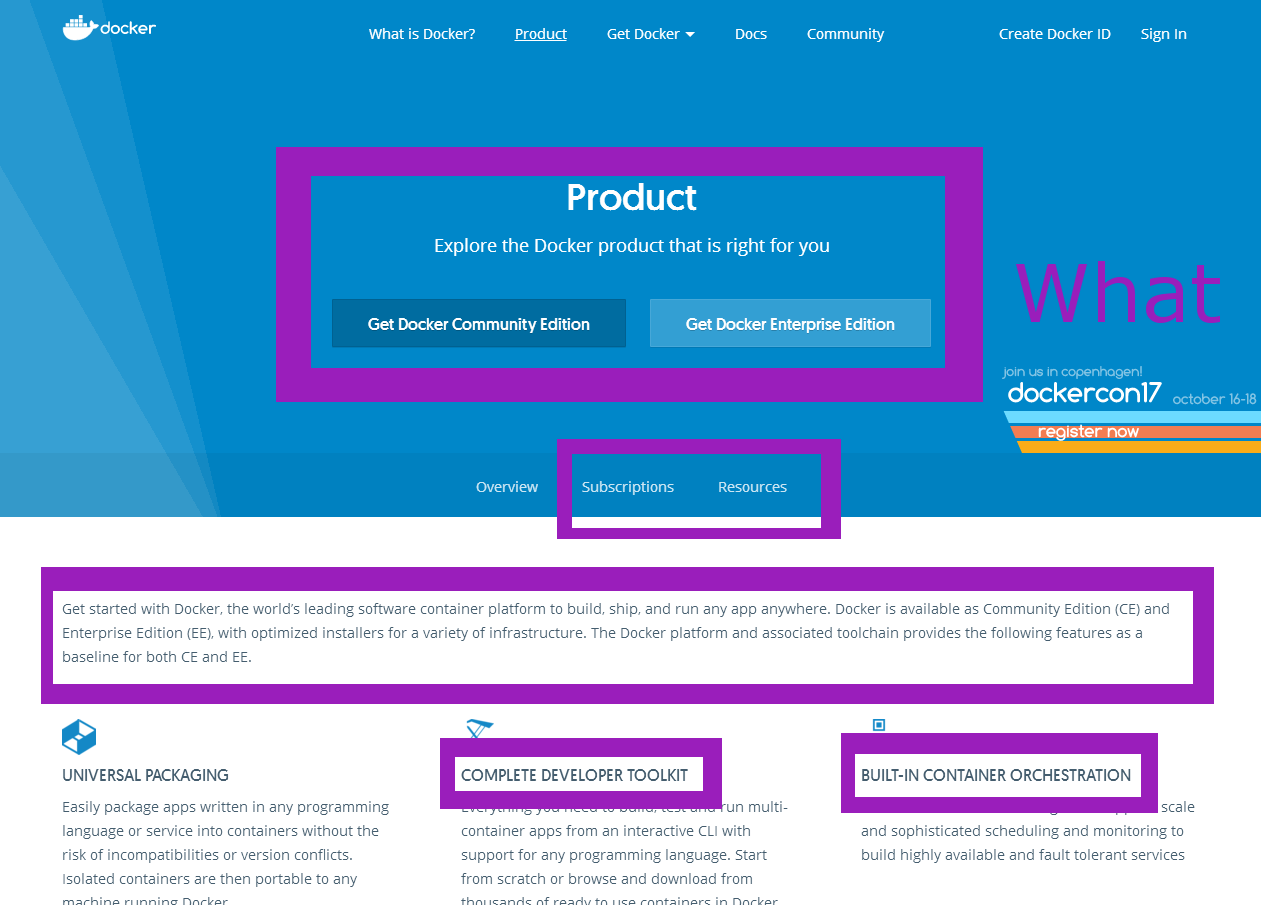
\includegraphics[width=\linewidth]{images/productwhat1.png}
    \label{fig:productwhat1}
    \caption{Individuazione What in product}
\end{figure}

\begin{figure}[H]
	\centering
	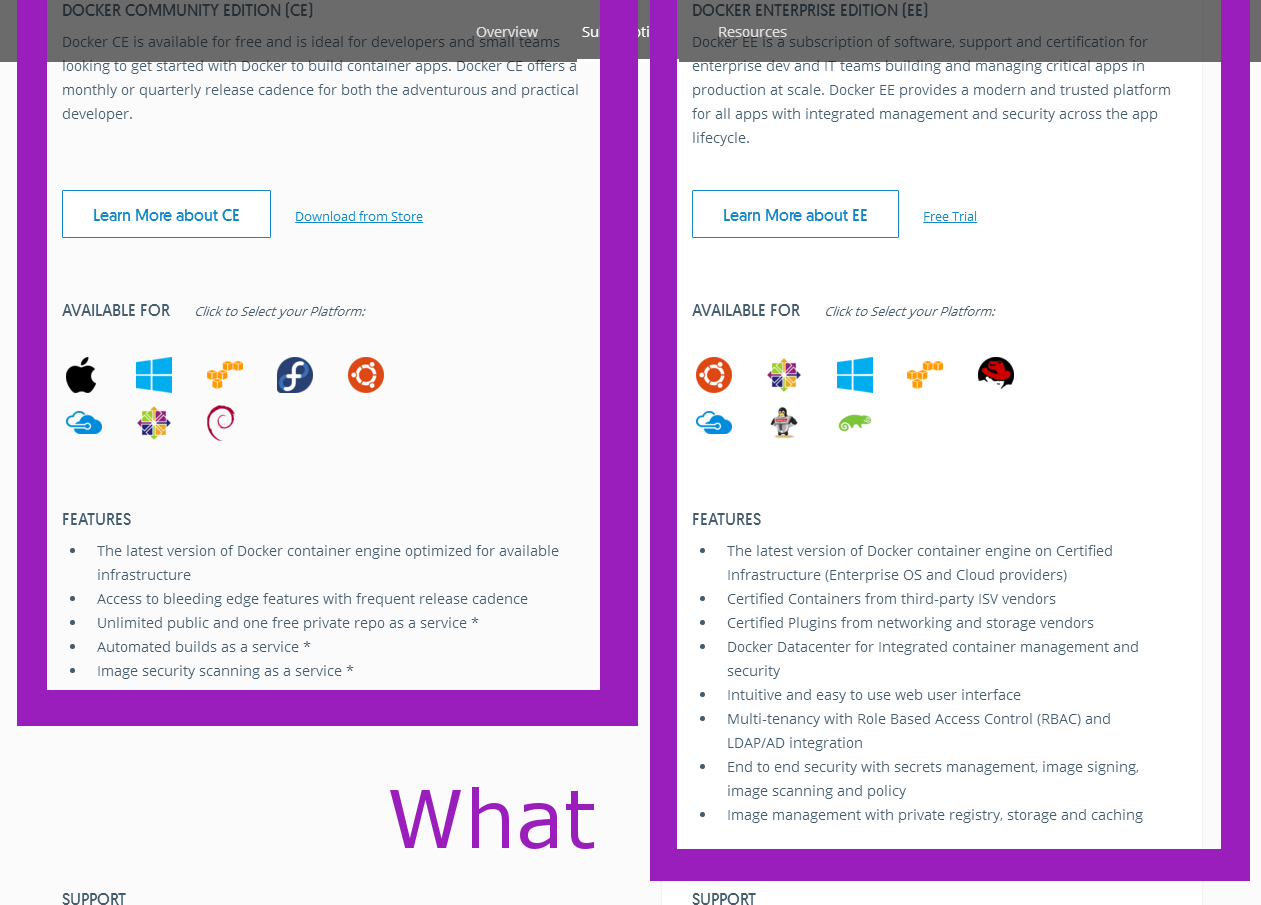
\includegraphics[width=\linewidth]{images/productwhat2.png}
    \label{fig:productwhat2}
    \caption{Individuazione What in product}
\end{figure}

\noindent La risposta è immediata. Presentare il proprio prodotto è esattamente lo scopo della pagina e lo esegue alla perfezione. Vengono elencate le caratteristiche di Docker, i due diversi software offerti e le loro differenze (piattaforme disponibili, features, prezzo e supporto).
\\
L'informazione è ben organizzata e chiara. Vari link conducono alle aree di approfondimento e di download.

\newpage
\subsubsection{Why?}
La domanda "Why?" corrisponde a "Perchè sono qui? Quali benefici ottengo dal sito?".
\\
Nelle pagine interne rispondere a tale domanda è opzionale.

\begin{figure}[H]
	\centering
	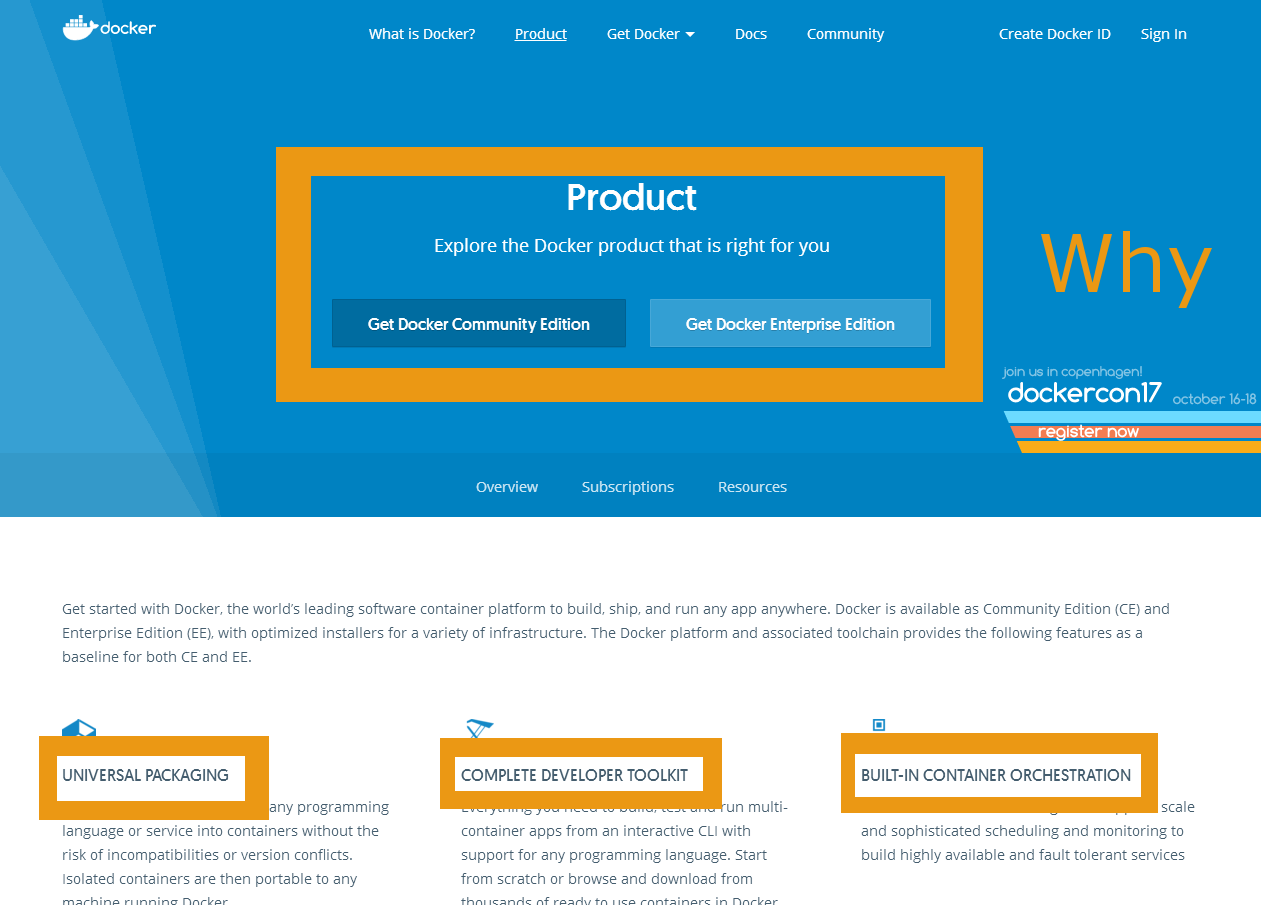
\includegraphics[width=\linewidth]{images/productwhy1.png}
    \label{fig:productwhy1}
    \caption{Individuazione Why in product}
\end{figure}

\begin{figure}[H]
	\centering
	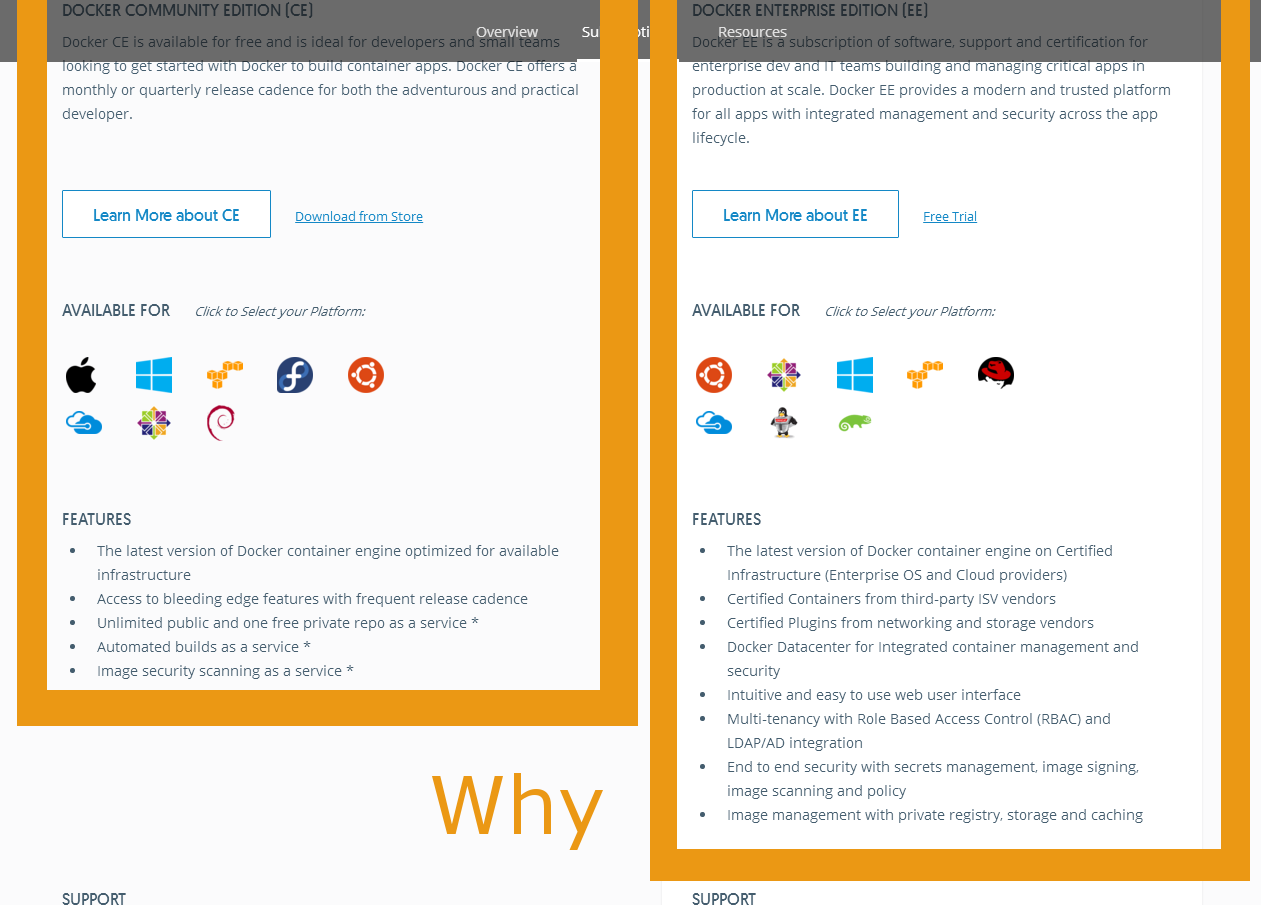
\includegraphics[width=\linewidth]{images/productwhy2.png}
    \label{fig:productwhy2}
    \caption{Individuazione Why in product}
\end{figure}

\noindent La risposta è chiara. I benefici che si ottengono dall'impiego di Docker per le proprio applicazioni sono descritti ampiamente in ogni parte del sito, compresa questa.
\\
La descrizione tra le due versioni di software offerto evidenzia molto accuratamente cosa ci si possa aspettare da Docker e la sua compatibilità con varie piattaforme è presentata bene come un punto di forza.

\subsubsection{When?}
La domanda "When?" corrisponde a "Quali sono le ultime novità del sito?".
\\
Nelle pagine interne rispondere a tale domanda è opzionale.

\begin{figure}[H]
	\centering
	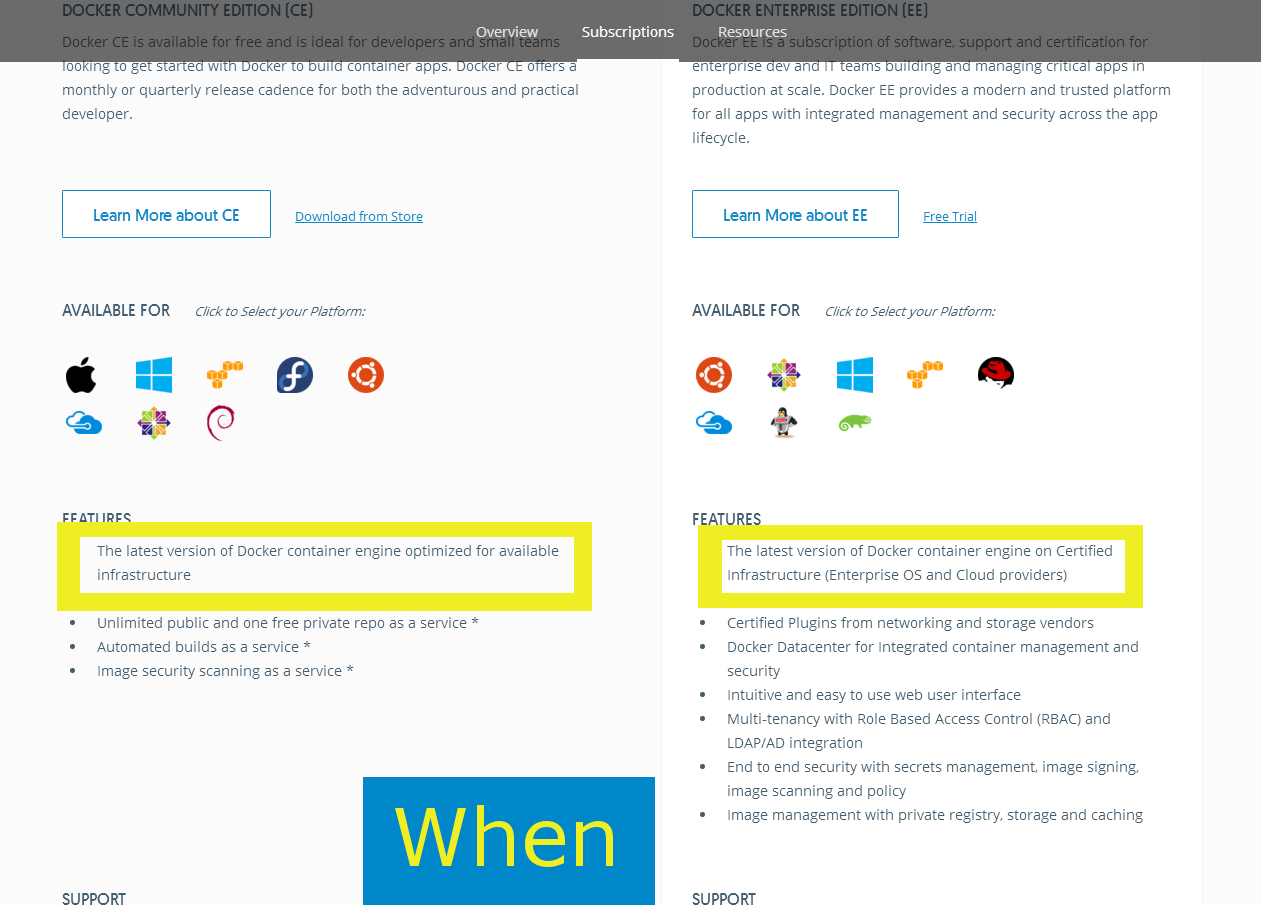
\includegraphics[width=\linewidth]{images/productwhen.png}
    \label{fig:productwhen}
    \caption{Individuazione When in product}
\end{figure}

\noindent La risposta non è immediata, visto che si trova in una frase assieme alle altre features. Viene dato per scontato, come in ogni sito di distribuzione diretta del proprio software, che la versione scaricabile sia la più recente e che siano utilizzati aggiornamenti automatici.

\subsubsection{How?}
La domanda "How?" corrisponde a "Come arrivo alle sezioni principali del sito?".
\\
Nelle pagine interne rispondere a tale domanda è opzionale.

\begin{figure}[H]
	\centering
	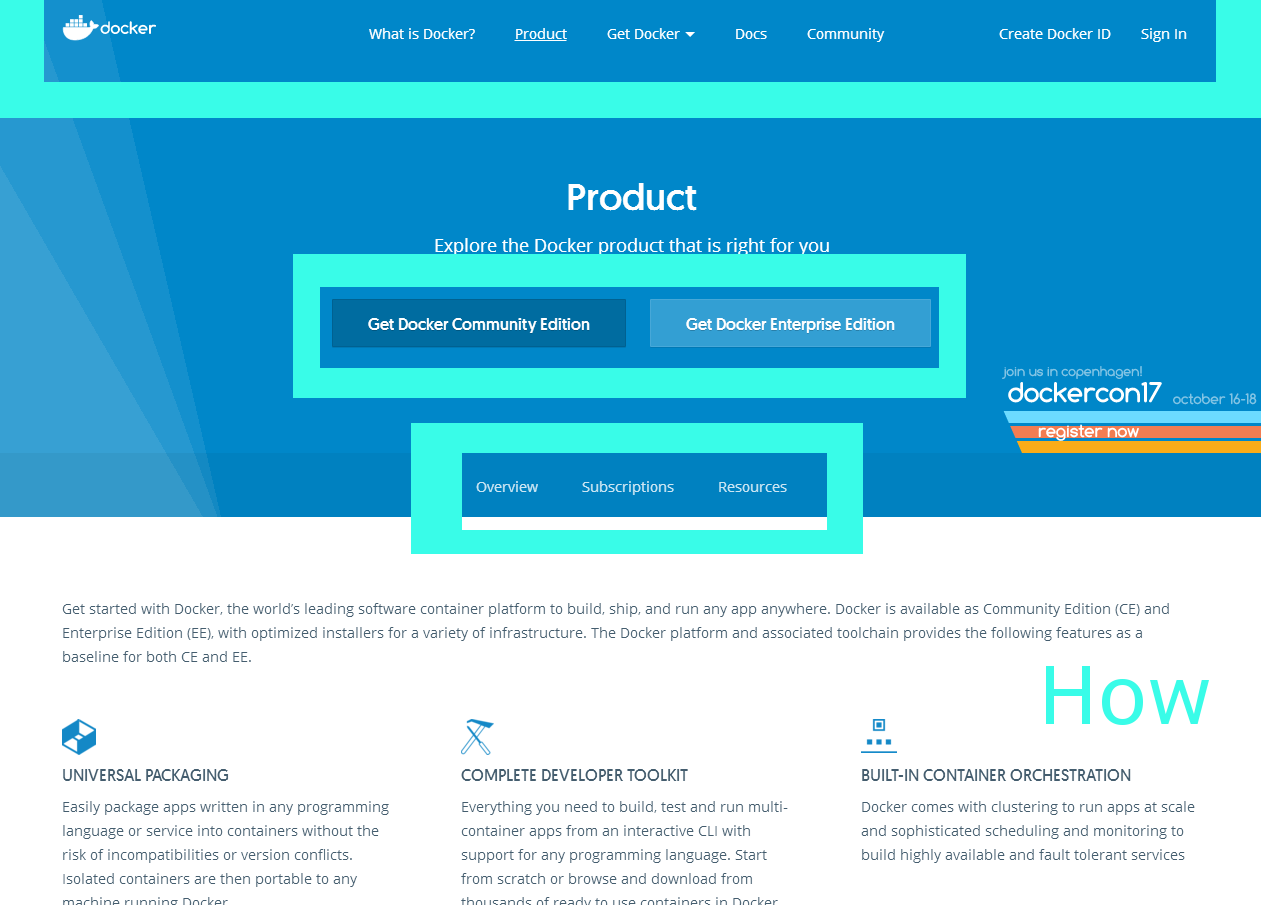
\includegraphics[width=\linewidth]{images/producthow1.png}
    \label{fig:producthow1}
    \caption{Individuazione How in product}
\end{figure}

\begin{figure}[H]
	\centering
	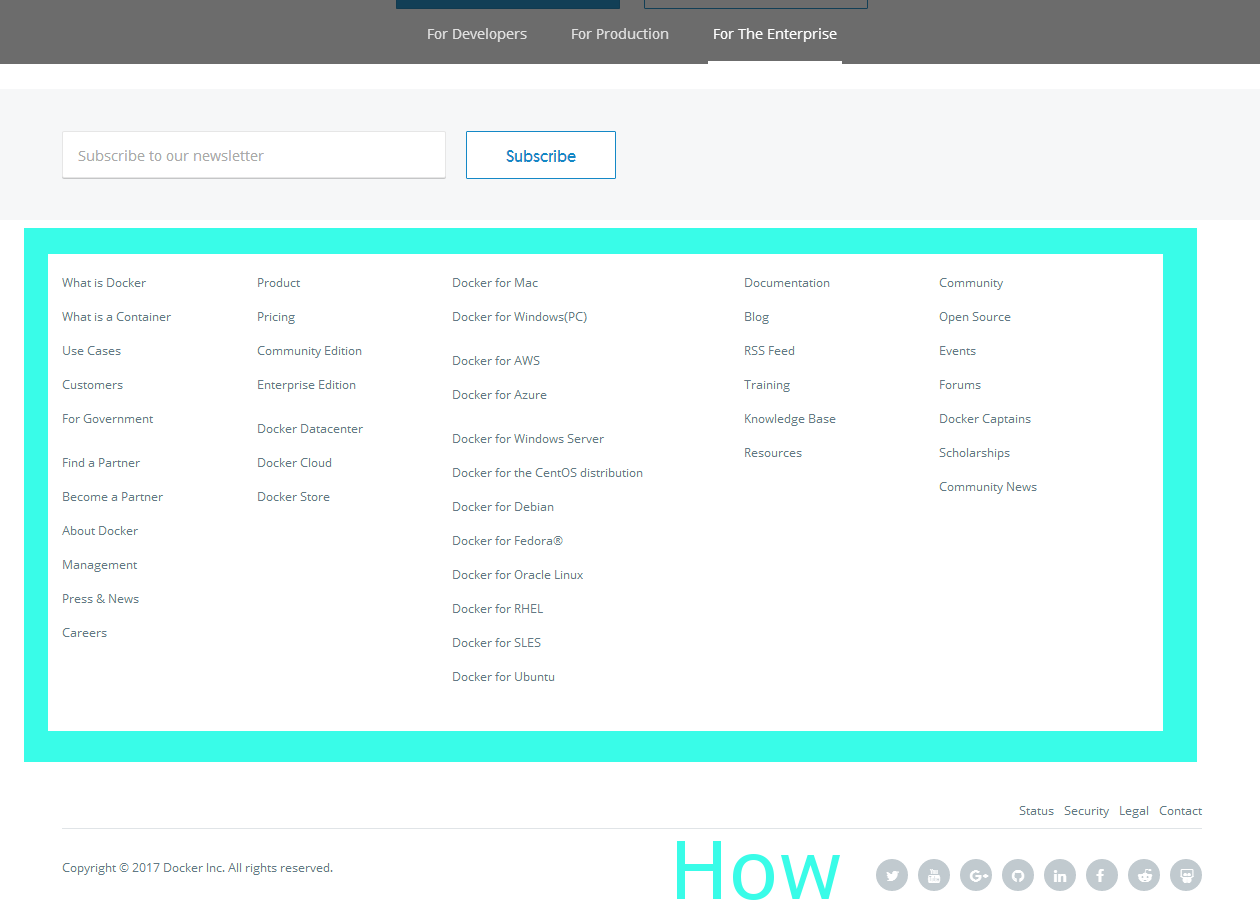
\includegraphics[width=\linewidth]{images/producthow2.png}
    \label{fig:producthow2}
    \caption{Individuazione How in product}
\end{figure}

\noindent La risposta è immediata. Gli elementi adibiti alla navigazione sono gli stessi della homepage, quindi le due breadcrumb, i pulsanti di approfondimento ed il footer svolgono efficacemente il loro ruolo.

\section{Analisi complessiva}

\subsection{Struttura}
La struttura del sito è ben organizzata. Poche pagine dense di contenuti separati in modo logico dal layout. Lo schema delle pagine è regolare, così da facilitare l'orientamento. Nessun elemento è troppo vicino o troppo lontano dai restanti, così da dimostrare ricchezza di contenuti ma senza causare claustrofobia.

\subsection{Navigazione}

\begin{figure}[H]
	\centering
	
\includegraphics[width=\linewidth]{images/breadcrumbinterna.png}
    \label{fig:breadcrumbint}
    \caption{Breadcrumb per la navigazione interna alla pagina}
\end{figure}

\noindent Ottima la breadcrumb per navigare all'interno della pagina, che continua a seguire l'utente durante lo scorrimento verticale, senza risultare ne' eccessiva ne' invasiva; inoltre la sua trasparenza evita sovrapposizioni sgradevoli.
\\
Tutti i link sono palesi (per la maggior parte sotto forma di pulsanti) ed anche se non si può verificare una precedente visita al link, la struttura estremamente semplice del sito compensa l'eventuale disagio.
\\
Potrebbe risultare difficoltoso leggere la breadcrumb centrale (per la navigazione interna alla pagina), visti il colore bianco/bluastro utilizzato per il testo.

\subsection{Pubblicità}
Essendo un sito che promuove il proprio prodotto, non è presente alcuna pubblicità esterna. L'unico elemento riconducibile ad una pubblicità, è la vetrina delle novità presente nella homepage. Tuttavia presenta solo informazioni ed eventi legati a Docker ed è un ottimo valore aggiunto per il sito e la sua professionalità.

\subsection{Immagini}
Nel sito web sono presenti poche immagini, con funzione perlopiù decorativa. Rispettano l'identità del prodotto, risultando affini a logo, colori ed ambito. Riempiono i buchi nel testo ed impediscono si formino muri di parole nei contenuti.
\\
L'immagine più rilevante è quella che compare nella homepage, in quanto animata. 

\begin{figure}[H]
	\centering
	
\includegraphics[width=\linewidth]{images/animalihomepage.png}
    \label{fig:animalianimati}
    \caption{Immagine animata della homepage}
\end{figure}

\noindent Ritrae due animaletti annoiati che, ricevuto un terminale con Docker, codificano allegramente. Nonostante la simpatia dell'animazione, è da considerare il rimpiazzo con un'immagine statica.
\\
E' comprensibile la volontà di incoraggiare l'utente a scorrere verticalmente la pagina, ma in questo modo l'attenzione passa dal prodotto all'immagine e rischia di rubare tempo prezioso. In alternativa, sarebbe consigliabile affiancarle dei contenuti più informativi come l'overview di Docker già presente in \url{https://www.docker.com/what-docker}, così da catturare l'attenzione e focalizzarla su ciò che è importante: il prodotto.

\subsection{Registrazione}
La registrazione non è obbligatoria e non viene forzata in alcun modo. Il visitatore, nel caso sia interessato a Docker e lo stia scaricando, dovrà registrarsi per utilizzarlo.
\\
L'operazione di "Sign In" conduce l'utente all'indirizzo \url{https://cloud.docker.com/swarm/<nomeutente>} e non è effettivamente possibile essere loggati in \url{https://www.docker.com/}.

\section{Altre pagine}
Le altre pagine presentate dal sito sono state escluse dall'analisi per almeno uno dei due principali motivi:

\begin{itemize}
	\item presentano gli stessi schemi delle pagine già analizzate, con simili pregi e difetti (Es: \url{https://www.docker.com/what-docker} è simile a \url{https://www.docker.com/});
    \item portano ad altri siti di Docker (Es: \url{https://docs.docker.com/};
    \item sono state scartate per scarso rapporto utilità/tempo (Es: \url{https://www.docker.com/docker-community}, che l'utente visita solo se veramente coinvolto e non propriamente per fattori di usabilità) in favore di maggior approfondimento nell'analisi.
\end{itemize}

\section{Considerazioni finali}
La pecca principale di \url{https://www.docker.com/}, nonchè un grave difetto, consiste nel contenuto della homepage. L'overview del prodotto dovrebbe essere tra le prime cose presentate, mentre è stata relegata ad una pagina interna.
\\
Dover effettuare un secondo click immediatamente dopo essere entrati nella homepage, causa fastidio a qualunque utente e non ci si può rifugiare dietro la scusa dell'esperienza informatica o della conoscenza pregressa del prodotto.
\\
Una pecca secondaria è la costrizione del visitatore a far uso massiccio di scroll verticale. In parte è comprensibile data la complessità del prodotto, tuttavia sarebbe opportuno adottare qualche misura a riguardo.
\\
Un approccio ragionevole sarebbe rinnovare l'homepage, rendendola più efficace nel descrivere l'attuale prodotto e più sintetica nelle descrizioni tecniche. Le descrizioni più tecniche verrebbero trasferite in \url{https://www.docker.com/what-docker}, cui il visitatore accederà con l'intenzione specifica di approfondire la sua conoscenza su Docker e sarà più disposto a scrollare la pagina.
\\
In aggiunta si potrebbe pensare ad una riduzione dell'ampiezza della vetrina delle novità (od il suo equivalente, nelle pagine interne).
\\
Non sono presenti altri problemi considerevoli o rilevanti; la struttura del sito è ordinata e la navigazione estremamente piacevole ed informativa.

\section{Giudizio finale}
Vengono riportati nella tabella i vari ambiti considerati nell'analisi e la loro valutazione. Segue il giudizio finale (che non è la semplice media delle varie valutazioni nella tabella) con un riassunto delle motivazioni.

\begin{table}[H]
\centering
\begin{tabular}{||l|r||}
\hline
Ambito & Voto \\ [0.5ex]
\hline \hline
Homepage Where? & 2/10 \\
Homepage Who? & 8/10 \\
Homepage Why? & 7/10 \\
Homepage What? & 4/10 \\
Homepage When? & 9/10 \\
Homepage How? & 9/10 \\
Product & 9/10 \\
Struttura & 9/10 \\
Immagini & 10/10 \\
Navigazione & 7/10 \\
Contenuti & 10/10 \\ [1.5ex]
Giudizio finale & 7/10 \\
\hline
\end{tabular}
\caption{Tabella del giudizio finale}
\end{table}

L'ostacolo principale del sito web di Docker è la necessità di esporre un prodotto complesso in breve tempo. Dal lato strutturale ed organizzativo si nota un lavoro perfetto. Dal lato informativo, i contenuti sono relativamente semplici e presentati con cura e chiarezza. La negligenza principale è di supporre che il visitatore conosca già perfettamente il prodotto e riesca così a navigare senza incidenti (o che sia troppo interessato per badare ad eventuali disagi). Appianata questa criticità, la valutazione di \url{https://www.docker.com/} risulterebbe superba.

\newpage
\section{Lista delle figure}

Per questioni di spazio, si useranno i seguenti termini nella colonna Sezione:
\begin{itemize}
	\item Homepage = \url{https://www.docker.com};
    \item Product = \url{https://www.docker.com/get-docker}.
\end{itemize}

\begin{table}[H]
\centering
\begin{tabular}{||c|c|c||}
\hline
Figura & File & Sezione \\ [0.5ex]
\hline \hline
logodocker & dockerlogo.jpg & / \\

homepage1 & homepage1.png & Homepage \\
homepage2 & homepage2.png & Homepage \\
homepage3 & homepage3.jpg & Homepage \\
homepage4 & homepage4.jpg & Homepage \\
homepage5 & homepage5.png & Homepage \\

homepagewhere & homepagewhere.png & Homepage \\
homepagewho & homepagewho.png & Homepage \\
homepagewhy & homepagewhy.png & Homepage \\
homepagewhat & homepagewhat.png & Homepage \\
homepagewhen & homepagewhen.png & Homepage\\
homepagehow1 & homepagehow1.png & Homepage \\
homepagehow2 & homepagehow2.png & Homepage \\
homepagehow3 & homepagehow3.png & Homepage \\

product1 & product1.png & Product \\
product2 & product2.png & Product \\
product3 & product3.png & Product \\
product4 & product4.png & Product \\
product5 & product5.png & Product \\

productwhere & productwhere.png & Product \\
productwho & productwho.png & Product \\
productwhat1 & productwhat1.png & Product \\
productwhat2 & productwhat2.png & Product \\
productwhy1 & productwhy1.png & Product \\
productwhy2 & productwhy2.png & Product \\
productwhen & productwhen.png & Product \\
producthow1 & producthow1.png & Product \\
producthow2 & producthow2.png & Product \\

breadcrumbint & breadcrumbinterna.png & Homepage \\
animalianimati & animalihomepage.png & Homepage \\
\hline
\end{tabular}
\caption{Tabella della lista delle figure}
\end{table}

\begin{thebibliography}{9}
\bibitem{usab}
	https://www.w3.org/WAI/intro/usable, articolo riguardante alcune parole chiave della Web Accessibility Initiative (WAI)
\bibitem{wsg}
  http://www.webstyleguide.com/wsg3/index.html, Web Style Guide 3rd Edition
\bibitem{eye}
	Eyetrack III, studio comportamentale sullo sguardo dei visitatori dei siti web
\end{thebibliography}

\end{document}